\documentclass[final,hidelinks,onefignum,onetabnum]{siamart250211}
%\documentclass[review,hidelinks,onefignum,onetabnum]{siamart250211}

\usepackage{amsfonts,amssymb}
%\usepackage{amsopn}
\usepackage{graphicx}
\ifpdf
  \DeclareGraphicsExtensions{.eps,.pdf,.png,.jpg}
\else
  \DeclareGraphicsExtensions{.eps}
\fi
\usepackage{bm}
%\usepackage{empheq}
%\usepackage{fancyvrb}
\usepackage{tikz}
\usetikzlibrary{math,positioning}

% Add a serial/Oxford comma by default.
\newcommand{\creflastconjunction}{, and~}

% Used for creating new theorem and remark environments
\newsiamremark{remark}{Remark}
\newsiamremark{stdass}{Standard Assumptions}
\newsiamthm{conjecture}{Conjecture}

\DeclareMathOperator{\diag}{diag}

\newcommand{\eps}{\epsilon}
\newcommand{\RR}{\mathbb{R}}

\newcommand{\grad}{\nabla}
\newcommand{\Div}{\nabla\cdot}

\newcommand{\bbf}{\mathbf{f}}
\newcommand{\bg}{\mathbf{g}}
\newcommand{\bn}{\mathbf{n}}
\newcommand{\bu}{\mathbf{u}}
\newcommand{\bv}{\mathbf{v}}
\newcommand{\bw}{\mathbf{w}}
\newcommand{\bx}{\mathbf{x}}
\newcommand{\bz}{\mathbf{z}}

\newcommand{\bU}{\mathbf{U}}
\newcommand{\bX}{\mathbf{X}}

\newcommand{\bzero}{\bm{0}}

\newcommand{\btau}{\bm{\tau}}

\newcommand{\cB}{\mathcal{B}}
\newcommand{\cH}{\mathcal{H}}
\newcommand{\cK}{\mathcal{K}}
\newcommand{\cQ}{\mathcal{Q}}
\newcommand{\cT}{\mathcal{T}}
\newcommand{\cV}{\mathcal{V}}
\newcommand{\cX}{\mathcal{X}}

\newcommand{\hcK}{\widehat{\cK}}

\newcommand{\nn}{{\text{\textnormal{n}}}}
\newcommand{\pp}{{\text{\textnormal{p}}}}
\newcommand{\qq}{{\text{\textnormal{q}}}}
\newcommand{\rr}{{\text{\textnormal{r}}}}

\newcommand{\ip}[2]{\left<#1,#2\right>}

\newcommand{\XX}{\ding{55}}

\newcommand{\dx}{\, \mathrm{d}x}

\newcommand{\rhoi}{\rho_{\text{i}}}

\DeclareMathOperator*{\argmin}{arg\,min}
\DeclareMathOperator*{\Hull}{Hull}

\newcommand{\Vdiv}{\cV_{\text{\textnormal{div}}}}

\newcommand{\CA}{C_\text{\textnormal{A}}}


% Optional PDF information
\ifpdf
\hypersetup{
  pdftitle={Surface elevation errors in finite element Stokes models for glacier evolution},
  pdfauthor={E. Bueler}
}
\fi

% Sets running headers as well as PDF title and authors
\headers{Surface elevation errors in Stokes models for glaciers}{E. Bueler}

% Title.
\title{Surface elevation errors in finite element Stokes models for glacier evolution\thanks{Submitted to the editors DATE (draft \today).  Thanks to J.~Ahlkrona and P.~Piersanti for thoughtful comments on an earlier version.}}

% Authors: full names plus addresses.
\author{Ed Bueler\thanks{Dept.~Mathematics \& Statistics, University of Alaska Fairbanks, USA (\email{elbueler@alaska.edu}, \href{https://bueler.github.io/}{\texttt{bueler.github.io}}).}}

% FundRef data to be entered by SIAM
%<funding-group specific-use="FundRef">
%<award-group>
%<funding-source>
%<named-content content-type="funder-name">
%</named-content>
%<named-content content-type="funder-identifier">
%</named-content>
%</funding-source>
%<award-id> </award-id>
%</award-group>
%</funding-group>


\begin{document}

\maketitle

\begin{abstract}
The primary data which determine the evolution of glaciation are the bedrock elevation and the surface mass balance.  From this data, which we assume is defined over a fixed land region, the glacier's geometry solves a free boundary problem which balances the time derivative of the surface elevation, the surface velocity from the very-viscous (Stokes) flow of the ice, and the surface mass balance.  This free boundary problem can be posed in weak form as a variational inequality over a convex set of admissible surface elevation functions, i.e.~those which are above the bedrock topography.  After some preparatory theory for the glaciological Stokes problem, we conjecture that a continuous-space, implicit time-step variational inequality problem for this surface elevation is well-posed if the surface kinematical equation is appropriately regularized.  This conjecture is supported by physical arguments and numerical evidence.  We prove a general theorem which bounds the numerical error made by finite element approximations of nonlinear-operator variational inequalities in Banach spaces.  The bound is a sum of error terms of different types, special to variational inequalities.  In the case of our implicit time-step glacier problem these terms are of three types: errors from discretizing the bed elevation, errors from numerically solving for the Stokes velocity, and finally an expected error which is quasi-optimal in the finite element representation of the surface elevation.
\end{abstract}

\begin{keywords}
error bounds, finite element methods, glaciers, ice flow, variational inequalities
\end{keywords}

\begin{MSCcodes}
76D27, 76D07, 49J40, 65N30, 65N15
\end{MSCcodes}


\section{Introduction} \label{sec:intro}

Glacier and ice sheet simulations model the ice as a free-surface layer of very-viscous, incompressible, and non-Newtonian fluid \cite{GreveBlatter2009,SchoofHewitt2013}.  Here we will only consider such simulations of land-based glaciers, without floating portions, and note that an ``ice sheet'' is simply a continent-scale glacier.  The two essential input data into such simulations are the bedrock elevation, which is assumed to be independent of time, and the time- and space-dependent surface mass balance rate (SMB).  By definition, the SMB is the balance between accumulating snow and the loss of melt water, through runoff, at the upper surface of the glacier \cite{Cogleyetal2011}.  Note that elevations are measured in meters, while SMB is in (ice-equivalent) meters per second.

Thus a glacier simulation takes, as inputs, the fixed bedrock topography, a variable SMB climate, and an initial glacier geometry.  The simulation produces the glacier's evolving geometry and flow velocity; these are the output fields of primary scientific value.  Comprehensive models  \cite{SchoofHewitt2013,Winkelmannetal2011}, however, have additional physics.  They might track the internal energy \cite{Aschwandenetal2012} or temperature of the ice, or liquid water at the top or bottom of the glacier.  For relative simplicity we only consider conservation of mass and momentum, but not energy, and liquid water plays no role.  Furthermore we will assume zero velocity at the base of the ice, a non-sliding and non-penetrating condition.  On the other hand, we will not make any shallowness assumptions \cite{SchoofHewitt2013}.

One may parameterize the glacier's geometry using either the (upper) surface elevation or the ice thickness.  Clearly, at a time and map-plane location where a glacier exists the surface elevation must exceed that of the bedrock, equivalently the ice thickness must be positive.  But then the computed flow velocity is only defined at those locations and times where ice is present, on the evolving 3D domain between the bedrock and surface elevations.  In other words, admissibility for the surface elevation is required merely to make the velocity and pressure Stokes problem meaningful.

Our notation is sketched in Figure \ref{fig:stokesdomain}.  Let $\Omega \subset \RR^2$ be a fixed portion of land, an open and connected set, with map-plane coordinates $x=(x_1,x_2)\in\Omega$.  All time-dependent quantities are assumed to be defined on $t\in [0,T]$ for some $T>0$.  We assume that we are given, as data, a real and continuous bed elevation function $b(x)$ on $\Omega$, and a real, signed, and continuous SMB function $a(t,x)$ on $[0,T]\times \Omega$.  Where $a>0$ (accumulation; downward arrows in Figure \ref{fig:stokesdomain}), a glacier will exist.  However, if $a<0$ (upward arrows) then either ice flow from accumulation areas has permitted a glacier to exist, with an ablating surface, or no glacier exists.  Determining which situation applies at some coordinates $t,x$ requires solving a free-boundary problems, as considered in this paper.

\begin{figure}[ht]
\centering
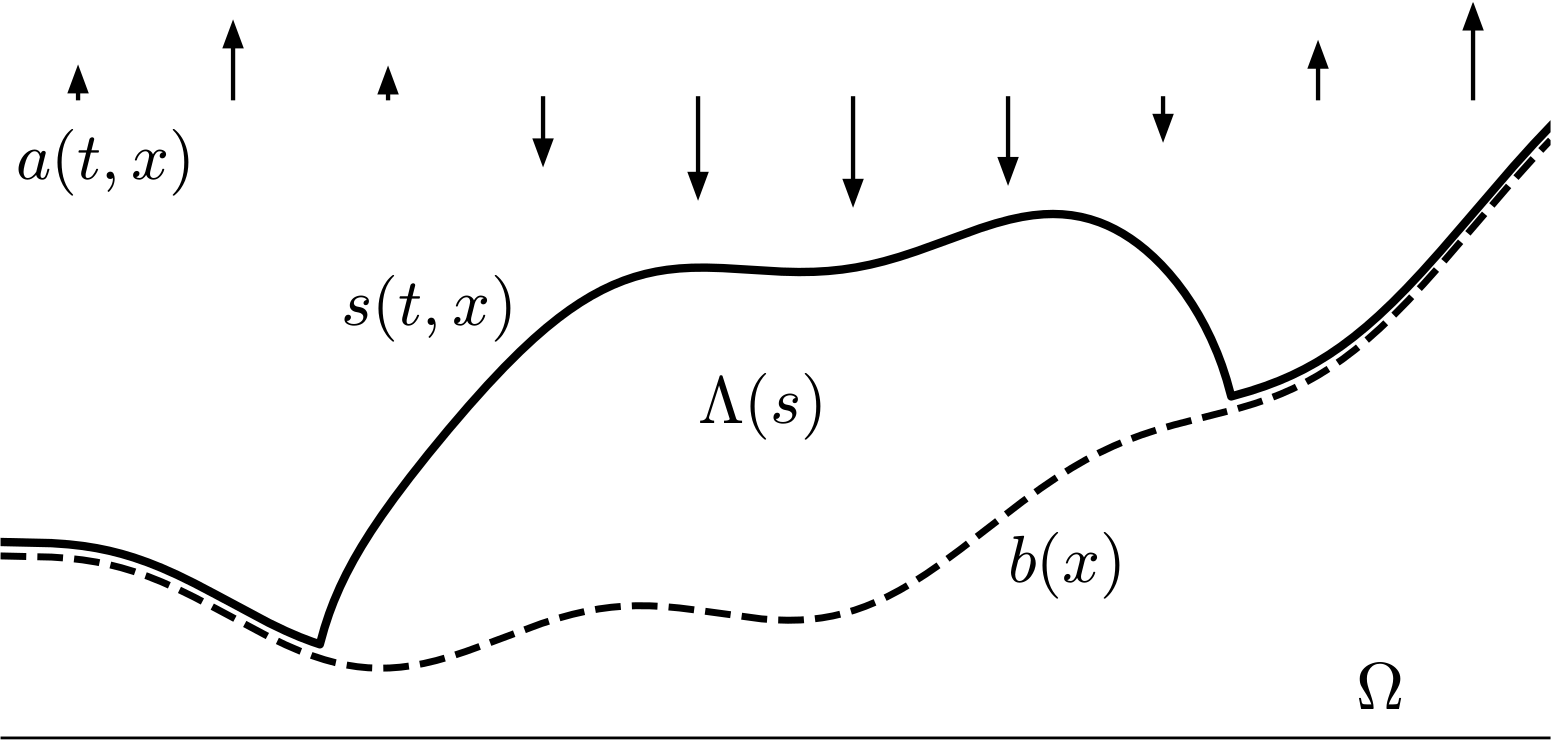
\includegraphics[width=0.6\textwidth]{genfigs/stokesdomain.pdf}
\caption{Glacier notation used in this paper; $x\in\Omega\subset\RR^2$ and $\Lambda(s)\subset\RR^3$.}
\label{fig:stokesdomain}
\end{figure}

Let $s(t,x)$ be the (solution) ice surface elevation.  We will regard this as defined for all $x\in\Omega$, but subject to the constraint that the surface $z=s$ must be at or above the bedrock ($s \ge b$).  In regions with no ice, $s=b$ holds.  The solution ice velocity $\bu(t,x,z)$ and pressure $p(t,x,z)$ are defined only on the open 3D domain
\begin{equation}
\Lambda(s) = \left\{(x,z)\,:\,b(x) < z < s(t,x)\right\} \subset \Omega \times \RR. \label{eq:icydomain}
\end{equation}
This aspect of glacier modeling deserves emphasis:  The time-dependent 3D domain $\Lambda(s)=\Lambda\big(s(t,x)\big)$, on which the velocity and pressure are meaningful, is determined by the evolving surface elevation $s$, which is itself part of the model solution.

The surface trace of the ice velocity will be of importance; a precise Sobolev space context is given in Section \ref{sec:stokes}.  We extend it by zero so that it is defined everywhere in $\Omega$:
\begin{equation}
\bu|_s(t,x) = \begin{cases} \bu(t,x,s(t,x)), & s(t,x)>b(t,x) \\
                            \bzero, & \text{otherwise} .\end{cases} \label{eq:defineus}
\end{equation}
(Compare flux extension by zero in \cite{SchoofHewitt2013}.)  Also let $\bn_s = \left<-\partial s/\partial x_1,-\partial s/\partial x_2,1\right>$ denote an un-normalized and upward surface normal vector, assumed well-defined for the purposes of this Introduction.  (Compare Section \ref{sec:model}.)

An infinite-dimensional nonlinear complementarity problem (NCP) \cite{FacchineiPang2003}, an obstacle problem, then applies almost everywhere in $[0,T]\times \Omega$:
\begin{subequations}
\label{eq:ncp}
\begin{align}
s - b &\ge 0 \label{eq:ncp:constraint} \\
\frac{\partial s}{\partial t} - \bu|_s \cdot \bn_s - a &\ge 0 \label{eq:ncp:residualpos} \\
(s - b) \left(\frac{\partial s}{\partial t} - \bu|_s \cdot \bn_s - a\right) &= 0
\end{align}
\end{subequations}
While condition \eqref{eq:ncp:constraint} is sometimes mentioned in the glaciers literature \cite{Durandetal2009,Halfar1981,JouvetBueler2012,PiersantiTemam2023,WirbelJarosch2020}, the complementary fact \eqref{eq:ncp:residualpos}, which says that a residual is everywhere nonnegative, observed first by \cite{Calvoetal2003}, is rarely written \cite{SchoofHewitt2013}.

System \eqref{eq:ncp} says that either a location is ice free ($s-b=0$), where the climate is locally ablating ($a\le 0$), or that the surface kinematical equation (SKE) holds:
\begin{equation}
\frac{\partial s}{\partial t} - \bu|_s \cdot \bn_s - a = 0.  \label{eq:ske}
\end{equation}
By \eqref{eq:ske} the (non-material) ice surface moves vertically according to the sum of the SMB and a component of the ice velocity at the surface \cite{SchoofHewitt2013}, which is a statement of mass conservation at the surface \cite{Aschwandenetal2012} called the free-surface equation \cite{LofgrenAhlkronaHelanow2022} or the kinematic boundary condition\footnote{Note that equation \eqref{eq:ske} is not a boundary condition of any identifiable PDE problem.} \cite{GreveBlatter2009}.  Glaciologists would agree with the conditions of NCP \eqref{eq:ncp} as a model for glaciers, though it may not be common to state it completely, as here.  In numerical ice sheet models the SKE \eqref{eq:ske} is a standard way for surface geometry to evolve \cite{GreveBlatter2009,SchoofHewitt2013}.  The idea that positive (continuous) SMB at a given location implies the existence of glacier ice is also not controversial, and ice-free conditions are well-understood to exist only where SMB is negative.

In the current paper the SMB $a$ is assumed to be defined everywhere in $\Omega$, regardless of whether a glacier is present or not.  Note that a simulated glacier needs to be able to advance, in a well-posed manner, into unglaciated locations.  In ice-free areas the input SMB should have the value which a glacier surface would experience at that time and location, which can be modeled using precipitation and an energy balance \cite{GreveBlatter2009}, for instance by hypothesizing an ice surface and computing the balance of snow accumulation minus ablation, using the energy available for melt.

After the kinematical considerations above, we can address non-shallow ice dynamics model used in this paper.  It is a standard approach which conserves mass and momentum, namely the non-sliding (e.g.~frozen) base, isothermal, non-Newtonian, and incompressible Stokes model \cite{GreveBlatter2009,JouvetRappaz2011,SchoofHewitt2013}, applied over the domain $\Lambda(s)$ defined in \eqref{eq:icydomain}.  Let $\Gamma_s \subset \partial \Lambda(s)$ be the upper surface $z=s$ and $\Gamma_b \subset \partial \Lambda(s)$ be the base $z=b$.  The possibility of cliffs at the ice margin is neglected, so $\partial \Lambda(s) = \overline{\Gamma_s} \cup \overline{\Gamma_b}$ is assumed to hold at any time.  (Section \ref{sec:theory} considers this aspect of the model.)  To state the shear-thinning constitutive relationship in the model, called Glen's flow law \cite{GreveBlatter2009}, let $D\bu=(\grad \bu + \grad \bu^{\top})/2$ denote the strain rate tensor, with Frobenius norm $|D\bu| = \left((D\bu)_{ij} (D\bu)_{ij}\right)^{1/2}$.  The effective ice (dynamic) viscosity \cite{GreveBlatter2009} is then given by a regularized formula
\begin{equation}
\nu(D\bu) = \nu_\pp \left(|D\bu|^2 + \eps\right)^{(\pp-2)/2} \label{eq:glen}
\end{equation}
for some $\eps>0$.  The exponent $1 < \pp \le 2$, often written $\pp=(1/\nn)+1$ in terms of Glen's exponent $n$, is approximately 4/3 in practice \cite{GreveBlatter2009}.  The coefficient $\nu_\pp>0$ has $\pp$-dependent units, while $\nu(D\bu)$ has SI units $\text{kg}\,\text{m}^{-1}\,\text{s}^{-1}$.  The values of $\nn$ and $\nu_\pp$ can be determined from measured properties of ice \cite{GoldsbyKohlstedt2001,GreveBlatter2009} and its temperature, but they are assumed to be constant here.  Note that $\pp=2$ yields a Newtonian fluid with constant viscosity, while for $\pp < 2$ the regularization implies that $\nu(D\bu)$ is bounded above.  The density of ice $\rhoi$ and the acceleration of gravity $\bg$ are also assumed constant.

In this Stokes model, at each time $t$ the velocity and pressure solve the following 3D fluid equations:
\begin{subequations}
\label{eq:stokes}
\begin{align}
- \nabla \cdot \left(2 \nu(D\bu)\, D\bu\right) + \nabla p &= \rhoi \bg && \text{within $\Lambda(s)$} \\
\nabla \cdot \bu &= 0 && \qquad \text{''} \label{eq:stokes:incomp} \\
\left(2 \nu(D\bu) D\bu - pI\right) \bn_s &= \bzero && \text{on $\Gamma_s$}\label{eq:stokes:stressfreesurface} \\
\bu  &= \bzero && \text{on $\Gamma_b$} \label{eq:stokes:noslide}
\end{align}
\end{subequations}
Boundary condition \eqref{eq:stokes:stressfreesurface} says that the sub-aerial upper surface is stress free; it must not be confused with the SKE \eqref{eq:ske}, though both apply on $\Gamma_s$.

In summary, at this point, we consider an evolving free-surface flow for a glacier, subject to a signed climate that can add or remove ice, simultaneously with a nonlinear Stokes problem which must be solved within the evolving 3D domain of ice.  This initial-boundary value problem, in strong form as \eqref{eq:icydomain}--\eqref{eq:stokes}, requires data $b(x)$ and $a(t,x)$, plus an initial surface elevation $s(0,x)$.  The solution variables are $s(t,x)$, $\bu(t,x,z)$, and $p(t,x,z)$, with $s$ defined everywhere over $[0,T]\times \Omega$, but subject to $s \ge b$, and with $\bu,p$ defined only on $\Lambda(s)$.  Note that NCP \eqref{eq:ncp} is the only part of the model where a time derivative appears.  Because the flow is very viscous \cite{Acheson1990}, the Stokes sub-model \eqref{eq:glen}--\eqref{eq:stokes} acts as an instantaneous ``algebraic'' constraint on the evolution statement \eqref{eq:ncp}.  This coupled and infinite-dimensional problem, for determining the evolving geometry of a glacier, is therefore simultaneously a differential algebraic equation (DAE) system \cite{AscherPetzold1998,LofgrenAhlkronaHelanow2022} and a free-boundary NCP.

While equivalent in many respects, formulations using thickness functions to parameterize glacier geometry have a different character from those using surface elevation as here.  The surface elevation $s$ is subject to a flow-caused smoothing effect, illustrated for a real ice sheet in Figure \ref{fig:giscross}.  For land-based glaciers $s(t,x)$ is generally smoother in $x$ than the thickness $H(t,x) = s(t,x)-b(x)$, because the latter ``inherits'' the lower regularity of the (typically) eroded bedrock topography $b$.

\begin{figure}
\begin{minipage}[t]{0.8\textwidth}
\vspace{0pt}
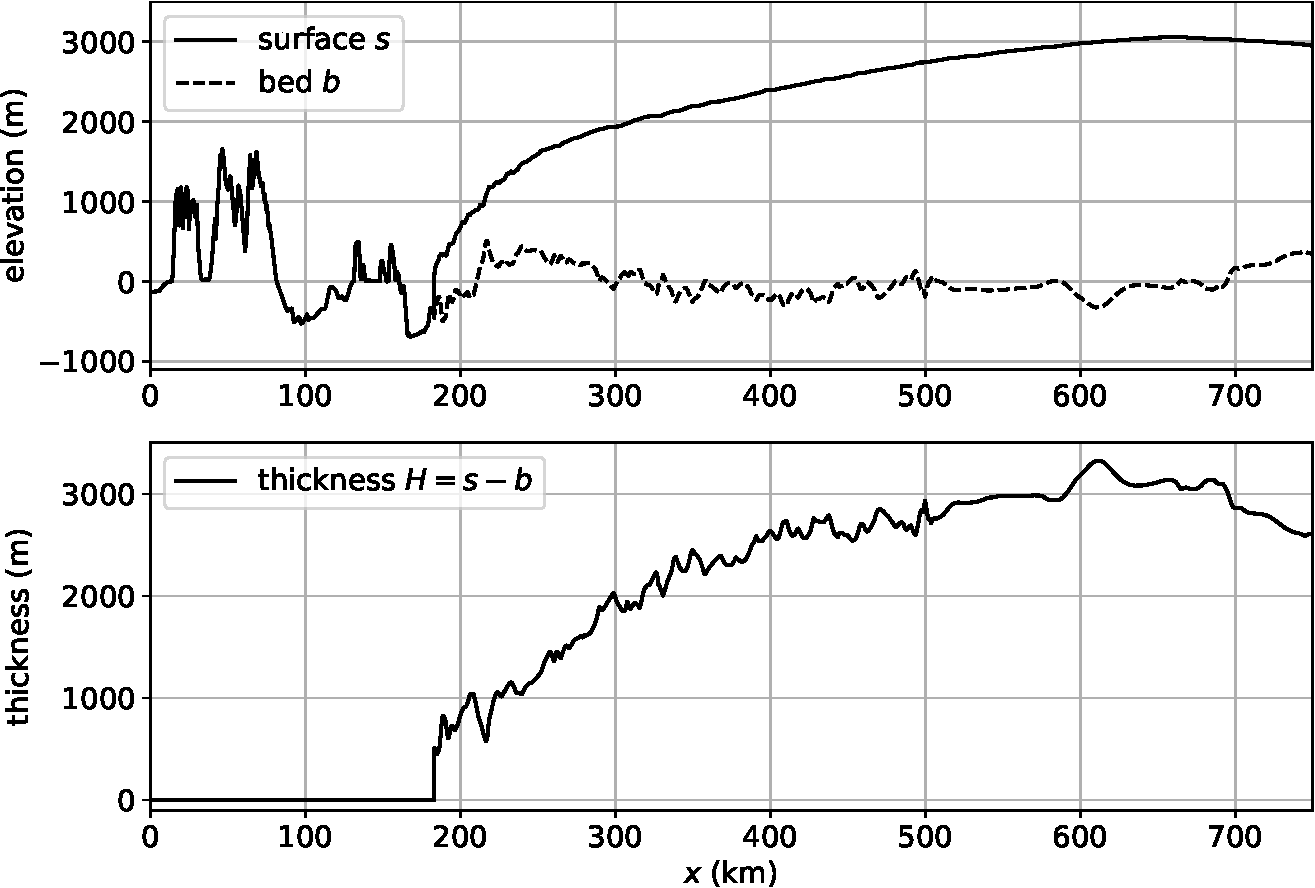
\includegraphics[width=\textwidth]{genfigs/giscross.pdf}
\end{minipage}
\,
\begin{minipage}[t]{0.15\textwidth}
\vspace{10pt}
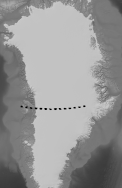
\includegraphics[width=\textwidth]{genfigs/gis/gris-profile-gray.png}
\end{minipage}
\caption{A cross-section of the Greenland ice sheet at $70^\circ$N latitude \cite{Morlighemetal2017}; see inset.  Top: While the ice surface $s$ is smoothed because of ice flow, the bedrock elevation $b$ is much rougher.  Bottom: The corresponding ice thickness $H = s-b$ inherits the low regularity of $b$.}
\label{fig:giscross}
\end{figure}

Glacier simulations are commonly discretized using a finite element (FE) approximation of the Stokes sub-problem \cite{IsaacStadlerGhattas2015,Jouvetetal2008,Pattynetal2008}.  However, to the author's knowledge all existing non-shallow evolution models, Stokes or otherwise, use an explicit or semi-implicit time-stepping scheme for the geometry, for example as in \cite{Brinkerhoff2023,Durandetal2009,Jouvetetal2008,LofgrenAhlkronaHelanow2022,WirbelJarosch2020}.  For these models which attempt implicitness, an important caveat is that the part of the map-plane domain covered by ice is not general, but is limited to an advance of one cell from the previous time step; in this sense (at least) these models are not fully implicit.

This work considers fully implicit time steps, as follows.  For a time step $\Delta t > 0$, the solution $s\approx s(t_n,x)$ to the backward Euler scheme for NCP \eqref{eq:ncp} satisfies
\begin{subequations}
\label{eq:be:ncp}
\begin{align}
s - b &\ge 0 \label{eq:be:ncp:constraint} \\
s - \Delta t\,\bu|_s \cdot \bn_s - \ell^n &\ge 0 \label{eq:be:ncp:residualpos} \\
(s - b) \left(s - \Delta t\,\bu|_s \cdot \bn_s - \ell^n\right) &= 0 \label{eq:be:ncp:complementarity}
\end{align}
\end{subequations}
which is also an NCP.  For clarity we have collected-together a source term $\ell^n(x) = s^{n-1}(x) + \int_{t_{n-1}}^{t_n} a(t,x)\,dt$, which must be assumed known when solving for $s$.  In Section \ref{sec:model} we re-write \eqref{eq:be:ncp} as a weak-form variational inequality (VI) for $s$ in a convex admissible subset of a Banach space.  Based on conjectured well-posedness for this problem (Section \ref{sec:theory}), our main results are then in Sections \ref{sec:abstractestimate} and \ref{sec:application}.  There we prove new estimates on the numerical error in an FE approximation of \eqref{eq:be:ncp}.

Note that an explicit time-step version of \eqref{eq:be:ncp} would replace the ``$s$'' symbols in the surface motion terms by the old surface elevation: $\bu|_s \cdot \bn_s \to \bu|_{s^{n-1}} \cdot \bn_{s^{n-1}}$ \cite{Lengetal2012}.  One possible semi-implicit scheme uses the surface velocity from the old time but the updated value for the surface slope part: $\bu|_s \cdot \bn_s \to \bu|_{s^{n-1}} \cdot \bn_s$ \cite{Durandetal2009}.  A different form of semi-implicitness comes from modifying the body force in the Stokes problem \cite{LofgrenAhlkronaHelanow2022}.  These schemes are distinct from fully-implicit scheme \eqref{eq:be:ncp}.

For a finite-dimensional DAE system an implicit scheme is the standard choice for handling their unbounded stiffness \cite{AscherPetzold1998}.  In the infinite-dimensional case here, where NCP \eqref{eq:ncp} is constrained at each time by the ``algebraic'' Stokes problem \eqref{eq:glen}--\eqref{eq:stokes}, implicit schemes are the natural choice (despite existing literature).  The backward Euler scheme in \eqref{eq:be:ncp} is merely the simplest A-stable scheme \cite{AscherPetzold1998} which can be applied to \eqref{eq:ncp}.  Extension to higher-order A-stable schemes, and/or stiff decay \cite{AscherPetzold1998} schemes, is natural and straightforward, but \eqref{eq:be:ncp} already contains all important features.

One might also make a case for implicit time-stepping based on simulation performance, that is, by computational complexity scaling arguments which compare to conditionally-stable explicit alternatives, as done by \cite{Bueler2023}.  However, any performance advantage depends on whether NCP \eqref{eq:be:ncp} is well-posed, whether it can be solved accurately, whether it can be solved efficiently, and also whether the implicit scheme turns out to have unconditional stability.  In the current paper we address well-posedness and FE accuracy for the weak form of \eqref{eq:be:ncp}.  Efficiency and time-stepping stability are topics for further research.

% FIXME remember to re-evaluate the next paragraph based on rewriting the whole paper and factoring stuff into appendices
This paper is organized as follows.  Section \ref{sec:stokes} recalls the theory of the Glen-law Stokes problem on a fixed domain.  For this sub-model we find an apparently-new bound on the surface trace of the velocity solution (Corollary \ref{cor:surfacetracebound}).  In Section \ref{sec:model} we reformulate the coupled, implicit-step NCP problem \eqref{eq:glen}--\eqref{eq:be:ncp} as a VI weak form.  The key coupling term is the surface motion term $\bu|_s\cdot \bn_s$ in SKE \eqref{eq:ske}, for which we provide a quantitative bound over a Sobolev space of surface elevation functions (Lemma \ref{lem:philipschitz}).  However, this bound is subject to Conjecture \ref{conj:a}, which hypothesizes that the surface velocity trace of the solution to \eqref{eq:glen}--\eqref{eq:stokes} is Lipschitz continuous with respect to surface elevation.  Well-posedness for each implicit step VI problem is considered in Section \ref{sec:theory}.  Certain physical and modeling ideas are discussed in this Section, as context needed to understand Conjecture \ref{conj:b}, which hypotheses the coercivity of a regularization of the surface motion term.  Next, in Section \ref{sec:numerical} we provide some numerical evidence for the validity of Conjecture \ref{conj:b}.  At this point we have in hand a mathematically-precise time-discretized model, though with only conjectural well-posedness; see Theorem \ref{thm:stepwellposed}.  This continuum model is apparently stated here for the first time.  Turning to FE approximations, in Section \ref{sec:abstractestimate} we prove an abstract FE error estimate, Theorem \ref{thm:abstractestimate} and its Corollaries, for general VI problems involving nonlinear operators on Banach spaces.  This new estimate, which makes coercivity and Lipshitz assumptions on the operator, extends the classical bilinear argument by Falk \cite{Falk1974}.  In Section \ref{sec:application} we apply the abstract estimate to the glacier problem, yielding our final result which is Theorem \ref{thm:glacierapp}.  The physical significance of each term in this error estimate, and how associated FE method and glacier modeling choices can be made, is addressed at the end.

We will use only the following few abbreviations: DAE (differential-algebraic equations), FE (finite element), NCP (nonlinear complementarity problem), PDE (partial differential equation), SKE (surface kinematical equation), SMB (surface mass balance), and VI (variational inequality).


\section{Surface velocity in a Stokes glacier model} \label{sec:stokes}

In this preparatory Section we address only the Stokes sub-model \eqref{eq:glen}--\eqref{eq:stokes}.  Applied on the 3D domain $\Lambda = \Lambda(s)$ defined by \eqref{eq:icydomain}, it computes the surface velocity $\bu|_s$ which appears in NCP \eqref{eq:ncp} or \eqref{eq:be:ncp}.  The ice base $\Gamma_b\subset\partial \Lambda$, on which the simple, non-sliding Dirichlet condition $\bu=\bzero$ holds, is assumed to have positive measure.  The remaining Neumann boundary $\Gamma_s = \partial \Lambda \setminus \overline{\Gamma_b}$ is subject to a zero normal stress condition.

Suitable function spaces for this sub-model are known.  Let $1 < \pp \le 2$.  Denote the Sobolev space \cite{Evans2010} of real-valued functions with $\pp$th-power integrable first derivatives by $W^{1,\pp}(\Lambda)$, and let $\cV = W_b^{1,\pp}(\Lambda; \RR^3)$ be the corresponding space of vector-valued functions with trace zero along $\Gamma_b$.  Let $[H]\ge 1\,\text{meter}$ be a representative \emph{vertical} glacier scale.  We define the norm on $\cV$ by
\begin{equation}
\|\bv\|_{\cV} = \left(\int_\Lambda |\bv|^\pp\,dx\,dz + [H]^\pp \int_\Lambda |\grad\bv|^\pp\,dx\,dz\right)^{1/\pp}. \label{eq:vnorm}
\end{equation}
The 3D volume element $dx\,dz = dx_1\,dx_2\,dz$ will be suppressed from now on.  Here $|\bv|$ denotes the Euclidean norm, and $|\grad\bv|=\left((\grad\bv)_{ij} (\grad\bv)_{ij}\right)^{1/2}$ is the Frobenius norm on $\RR^{3\times 3}$.  Length scaling $[H]$ gives $\|\bv\|_{\cV}$ consistent units; compare \cite[Remark 1.2.1]{BoffiBrezziFortin2013}.  Let $\cQ=L^{\pp'}(\Lambda)$ where $\pp'=\pp/(\pp-1)$ is the conjugate exponent.  Define $\mathcal{M} = \cV \times \cQ$ as the space of admissible velocity and pressure pairs.  For $(\bu,p), (\bv,q) \in \mathcal{M}$ define
\begin{equation}
F_\Lambda(\bu,p)[\bv,q] = \int_\Lambda 2 \nu(D\bu) D\bu : D\bv - p \Div\bv - (\Div\bu) q - \rhoi \bg \cdot \bv, \label{eq:glenstokes:fcnl}
\end{equation}
where $A:B=a_{ij}b_{ij}$.  The (mixed) weak form of the Stokes sub-model \eqref{eq:glen}--\eqref{eq:stokes} now seeks the solution $(\bu,p) \in \mathcal{M}$ satisfying
\begin{equation}
F_\Lambda(\bu,p)[\bv,q] = 0 \qquad \text{for all } (\bv,q) \in \mathcal{M}. \label{eq:glenstokes:weak}
\end{equation}

Jouvet and Rappaz \cite{JouvetRappaz2011} have proven that problem \eqref{eq:glenstokes:weak} is well-posed if the Neumann portion of $\partial\Lambda$ is $C^1$.  Their proof uses the equivalence of \eqref{eq:glenstokes:weak} and a minimization problem over the divergence-free subspace $\Vdiv = \{\bv\in\cV\,:\,\Div\bv=0\}$.  Our regularization in Glen law \eqref{eq:glen} differs from that in \cite{JouvetRappaz2011}, but the necessary modifications are addressed in \cite{Belenkietal2012,IsaacStadlerGhattas2015}.  Note that if the weak solution is sufficiently regular then the strong form \eqref{eq:stokes} is also satisfied.

\begin{theorem}[Theorem 3.10 in \cite{JouvetRappaz2011}] \label{thm:stokeswellposed}  Suppose $\Lambda$ is bounded, $\partial\Lambda$ is Lipschitz, $\Gamma_s$ is $C^1$, and $\Gamma_b$ has positive measure.  Let $1<\pp\le 2$ and $\eps>0$ in \eqref{eq:glen}.  Then there exists a unique pair $(\bu,p) \in \mathcal{M}$ solving \eqref{eq:glenstokes:weak}, and $\bu\in \Vdiv$.
\end{theorem}

Our primary purpose is to study NCP \eqref{eq:be:ncp} for the glacier geometry, and its weak form, but for that we need to bound the surface trace $\bu|_s$.  The following \emph{a priori} bound, proven for completeness in Appendix \ref{app:provestokesapriori}, shows that the velocity solution is controlled by certain physical constants and the geometry of $\Lambda$.

\begin{lemma} \label{lem:stokesapriori}
There is $C>0$ depending continuously on $\pp$, $\rhoi |\bg|$, $\nu_\pp$, $\eps$, $[H]$, and $\Lambda$ so that if $\bu\in\cV$ is the solution from Theorem \ref{thm:stokeswellposed} then
\begin{equation}
\|\bu\|_{\cV} \le C. \label{eq:stokesapriori}
\end{equation}
\end{lemma}

\begin{lemma}[Trace inequality] \label{lem:trace}
Under the assumptions of Theorem \ref{thm:stokeswellposed}, there exists a constant $C$, dependent only on $\pp$, $[H]$, and $\Lambda$, so that for all $\bv \in \cV$,
\begin{equation}
\int_{\Gamma_s} |\bv|^\pp \,dS \le C \|\bv\|_{\cV}^\pp. \label{eq:trace}
\end{equation}
On the left of \eqref{eq:trace}, $\bv$ denotes the trace on $\Gamma_s$ and $dS$ is the area element over $\partial\Lambda$.
\end{lemma}

\begin{proof}
Theorem 5.5.1 in \cite{Evans2010} defines the trace operator $T:\cV\to L^\pp(\partial\Lambda)$, for which there exists a constant $c>0$ so that
\begin{equation}
\int_{\partial\Lambda} |T\bv|^p\,dS \le c \int_{\Lambda} |\bv|^\pp + |\grad\bv|^\pp \le c \int_{\Lambda} |\bv|^\pp + [H]^\pp |\grad\bv|^\pp \label{eq:tracework}
\end{equation}
for $\bv\in\cV$.  However, because $\bv=\bzero$ along $\Gamma_b$, and by the Poincar\'e inequality \eqref{eq:poincare}, the result follows.
\end{proof}

Combining Lemmas \ref{lem:stokesapriori} and \ref{lem:trace} yields the following bound on the surface trace of the velocity.  In using this result, recall that $\Lambda=\Lambda(s)$ and $\Gamma_s=\partial \Lambda\setminus \Gamma_b$ are defined, in terms of $s$ and $b$, by \eqref{eq:icydomain}.

\begin{corollary}[Surface velocity bound] \label{cor:surfacetracebound}
There is a constant $C>0$, computable from physical constants and the geometry of $\Lambda$, so that if $\bu\in\cV$ is the Stokes velocity solution from Theorem \ref{thm:stokeswellposed} then
\begin{equation}
\int_{\Gamma_s} |\bu|^\pp \,dS \le C. \label{eq:surfacetracebound}
\end{equation}
\end{corollary}


\section{The weak-form implicit time-step model} \label{sec:model}

Now we return to implicit time steps for the surface elevation, in a model based on Stokes dynamics and NCP \eqref{eq:be:ncp}.  Let $\{t_n\}$ be any increasing sequence of times in $[0,T]$, with $t_0=0$.  Let $\Delta t = t_n-t_{n-1}$ denote a step length, and let $a^n(x)$ be the (temporal) average of the data $a(t,x)$ over $[t_{n-1},t_n]$.  Suppose that $s(x)=s^n(x)\approx s(t_n,x)$ approximates the surface elevation at time $t_n$.  Using a backward Euler implicit step \cite{AscherPetzold1998}, SKE \eqref{eq:ske} becomes
\begin{equation}
\frac{s - s^{n-1}}{\Delta t} - \bu|_{s} \cdot \bn_{s} - a^n = 0; \label{eq:be:ske}
\end{equation}
this is the basis for NCP \eqref{eq:be:ncp}.  This scheme is fully implicit because the unknown $s=s^n$ appears both in the surface velocity $\bu|_s$ and the slope $\bn_s$.  For cleaner appearance we clear the denominator in \eqref{eq:be:ske} and collect a source term:
\begin{equation}
\ell^n(x) = s^{n-1}(x)+\Delta t\,a^n(x) = s^{n-1}(x) + \int_{t_{n-1}}^{t_n} a(t,x)\,dt. \label{eq:be:source}
\end{equation}

As noted in the Introduction, $s=s^n$ in \eqref{eq:be:ske} actually solves a problem of free-boundary type, NCP \eqref{eq:be:ncp}.  Complementarity condition \eqref{eq:be:ncp:complementarity} says that, at the solution time, and almost everywhere over $\Omega$, either there is no ice ($s=b$) or equation \eqref{eq:be:ske} holds.  Of course, $s$ does not solve \eqref{eq:be:ske} over the bare ground part of $\Omega \subset \RR^2$, where $s=b$, but it solves all parts of \eqref{eq:be:ncp}.

The strong form NCP \eqref{eq:be:ncp} has a weak-form variational inequality (VI; \cite{Evans2010,KinderlehrerStampacchia1980}) version which is better-suited to both well-posedness theory and finite element (FE) analysis.  Let us regard the precise Banach space $\cX$ of surface elevations as unknown for now.  Admissible surface elevations for the weak formulation come from a convex and closed subset,
\begin{equation}
\cK = \left\{r \in\cX\,:\,r|_{\partial\Omega}=b|_{\partial\Omega} \text{ and } r \ge b\right\};  \label{eq:be:admissible}
\end{equation}
note this includes the fixed (Dirichlet) boundary condition.

The VI is derived as follows; compare \cite{Bueler2021conservation}.  Suppose that $s \in \cK$ is a sufficiently-regular solution of NCP \eqref{eq:be:ncp}.  Let $\Omega_I$ be the (measurable) subset of $\Omega$ on which constraint \eqref{eq:be:ncp:constraint} is inactive, i.e.~where glacier ice is present: $\Omega_I = \{x\,:\,s(x)>b(x)\}$.  From \eqref{eq:be:ncp:complementarity}, integration over $\Omega_I$ shows that
\begin{equation}
\int_{\Omega_I} \left(s - \Delta t\,\bu|_s \cdot \bn_s - \ell^n\right)\,(r-s) = 0  \label{eq:inactivetruth}
\end{equation}
for any $r\in\cK$.  On the other hand, let $\Omega_A = \{x \in \Omega \,:\,s(x)=b(x)\}$ be the complementary active (ice-free) region.  Observe that \eqref{eq:be:ncp:residualpos} says that $b-\ell^n = s - \Delta t\,\bu|_s \cdot \bn_s - \ell^n \ge 0$ on $\Omega_A$,\footnote{Note the role of extension by zero \eqref{eq:defineus} here.} and that $r-s=r-b\ge 0$ on $\Omega_A$ if $r\in\cK$.  Therefore integration of the same quantity as in \eqref{eq:inactivetruth} now yields an inequality:
\begin{equation}
\int_{\Omega_A} \left(s - \Delta t\,\bu|_s \cdot \bn_s - \ell^n\right)\,(r-s) = \int_{\Omega_A} \left(b - \ell^n\right)\,(r-b) \ge 0.  \label{eq:activetruth}
\end{equation}
Almost everywhere, either land is glacier covered (within $\Omega_I$) or ice-free ($\Omega_A$), so addition of \eqref{eq:inactivetruth} and \eqref{eq:activetruth} gives the following VI for $s \in \cK$:
\begin{equation}
\int_\Omega \left(s - \Delta t\,\bu|_s \cdot \bn_s - \ell^n\right)\,(r-s) \ge 0 \quad \text{for all } r \in \cK. \label{eq:be:viearly}
\end{equation}
This integral inequality is known to be true for $s\in\cK$, in advance of any knowledge about where is the ice-covered part of $\Omega$.
	
Well-posedness of the weak-form Stokes problem \eqref{eq:glenstokes:weak} over a 3D domain $\Lambda$, plus the surface trace bound in Corollary \ref{cor:surfacetracebound}, allows us to create a well-defined map from an admissible surface elevation $s$ to the corresponding surface velocity solution $\bu|_s$.  The map is defined via \eqref{eq:icydomain} for $\Lambda=\Lambda(s)$, followed by the solution of \eqref{eq:glenstokes:weak} over $\Lambda$, evaluation of the trace of $\bu$ along $\Gamma_s$ (Corollary \ref{cor:surfacetracebound}), and then definition \eqref{eq:defineus}, which includes extension by zero.  For this to be well-defined, $s$ must be admissible ($s\in\cK$) and sufficiently regular.  We call
\begin{equation}
\Phi(s) = - \bu|_s\cdot \bn_s \label{eq:definePhi:asfunction}
\end{equation}
the \emph{surface motion map}.  It maps a scalar surface elevation function $s$ to the dynamical term in the SKE \eqref{eq:be:ske} and the NCP \eqref{eq:be:ncp}.

Constructing a bound for $\Phi$ will help to identify a Banach space $\cX$ in which to seek admissible solutions $s$.  As before, let $\Omega \subset \RR^2$ be a bounded domain.  Let $[L]>0$ be a representative \emph{horizontal} scale; compare \eqref{eq:vnorm}.  For $q\in W^{1,\rr}(\Omega)$ we define
\begin{equation}
\|q\|_{W^{1,\rr}} = \left(\int_\Omega |q|^\rr\,dx + [L]^\rr \int_\Omega |\grad q|^\rr\,dx\right)^{1/\rr}. \label{eq:norm:Omega}
\end{equation}
The key assumption in the following Lemma is that $s\in W^{1,\rr}(\Omega)$ implies that the domain $\Lambda=\Lambda(s)$ is nice enough so that Corollary \ref{cor:surfacetracebound} gives a finite bound.  The key conclusion is that $\Phi(s) \in \left(W^{1,\rr}(\Omega)\right)'$, the dual space, which will be critical in analyzing the weak form of NCP \eqref{eq:be:ncp}.

\begin{lemma}[Preliminary bound on $\Phi(s)$] \label{lem:phibound:early}  Suppose $2 \le \rr \le \infty$, and assume $s\in W^{1,\rr}(\Omega)$ is admissible, $s\ge b$.  With $\Lambda(s)$ defined by \eqref{eq:icydomain}, assume that the hypotheses of Theorem \ref{thm:stokeswellposed} and Corollary \ref{cor:surfacetracebound} apply, thus that $\Phi(s)$ is a well-defined measurable function.  Then there is $C>0$, depending on $s$ and $\bu|_s$ but not $q$, so that
\begin{equation}
\left|\int_\Omega \Phi(s) q\,dx\right| = \left|\int_\Omega \bu|_s\cdot \bn_s q\,dx\right| \le C\, \|q\|_{W^{1,\rr}} \qquad \text{for all } q\in W^{1,\rr}(\Omega).  \label{eq:phibound:early}
\end{equation}
\end{lemma}

\begin{proof}  Observe that $dS = |\bn_s|\,dx = \sqrt{1+|\grad s|^2}\,dx$ is the surface area element for $\Gamma_s \subset \partial \Lambda$.  Apply the triangle, Cauchy-Schwarz, and H\"older's inequalities (H\"older twice):
\begin{align}
\left|\int_\Omega \Phi(s) q\,dx\right| &\le \int_\Omega \big|\bu|_s\big| |\bn_s| |q|\,dx = \int_\Omega \big|\bu|_s\big| |\bn_s|^{1/\pp} |\bn_s|^{1/\pp'} |q|\,dx \label{eq:phibound:zero} \\
    &\le \left(\int_\Omega \big|\bu|_s\big|^\pp |\bn_s|\,dx\right)^{1/\pp} \left(\int_\Omega |\bn_s| |q|^{\pp'} \,dx\right)^{1/\pp'} \notag \\
    &\le \left(\int_{\Gamma_s} |\bu|^\pp \,dS\right)^{1/\pp} \left(\int_\Omega |\bn_s|^\rr \,dx\right)^{1/(\pp'\rr)} \left(\int_\Omega |q|^{\pp'\rr'} \,dx\right)^{1/(\pp'\rr')}. \notag
\end{align}
If $C_1$ is the \emph{a priori} bound from \eqref{eq:surfacetracebound} then
\begin{equation}
\left|\int_\Omega \Phi(s) q\,dx\right| \le C_1^{1/\pp} \left(\int_\Omega \left(1+|\grad s|^2\right)^{\rr/2}\,dx\right)^{1/(\pp'\rr)} \|q\|_{L^{\pp'\rr'}}.
\end{equation}
Note that if $\alpha\ge 0$ then $(1+\alpha)^{\rr/2} \le 2^{(\rr-2)/2} (1+\alpha^{\rr/2})$, so
\begin{align}
\left|\int_\Omega \Phi(s) q\,dx\right| &\le C_1^{1/\pp} \left(2^{(\rr-2)/2} \int_\Omega 1 + |\grad s|^\rr\,dx\right)^{1/(\pp'\rr)} \|q\|_{L^{\pp'\rr'}} \label{eq:phibound:one} \\
  &\le C_2 \left(|\Omega| + [L]^{-\rr}\|s\|_{W^{1,\rr}}^\rr\right)^{1/(\pp'\rr)} \|q\|_{L^{\pp'\rr'}}. \notag
\end{align}
Since $2 \le \pp' \le \pp'\rr' < \infty$, by Sobolev's inequality\footnote{For example, apply Theorem 8.8 from \cite{LiebLoss1997} using $n=2$, $k=m=1$, $p=\rr$, and $q=\pp'\rr'$.} we also have $\|q\|_{L^{\pp'\rr'}} \le C_3 \|q\|_{W^{1,\rr}}$, which yields \eqref{eq:phibound:early}.
\end{proof}

The measurable function $\bu|_s$ may be discontinuous on $\Omega$, but, based on the above result, we now conjecture that for some $\rr>2$, the $L^{\rr'}$-norm of $\bu|_s$ is Lipschitz as a function of $s \in W^{1,\rr}(\Omega)$.  The reason for requiring $\rr>2$ will be seen in Lemma \ref{lem:philipschitz}; this would seem to be a technical requirement.

\begin{conjecture}[Surface velocity is a Lipschitz function of surface elevation] \label{conj:a}

\noindent There exists $2 < \rr \le \infty$ with the following two properties:  \emph{(i)} If $s\in W^{1,\rr}(\Omega)$ is admissible ($s\ge b$ and $s=b$ on $\partial\Omega$) then the conclusion of Theorem \ref{thm:stokeswellposed} applies, giving a well-defined surface velocity $\bu|_s$.  \emph{(ii)} There exists $C>0$, independent of (admissible) $s,r\in W^{1,\rr}(\Omega)$, such that
\begin{equation}
\big\|\bu|_r - \bu|_s\big\|_{L^{\rr'}} \le C \|r-s\|_{W^{1,\rr}}. \label{eq:ulipschitz}
\end{equation}
\end{conjecture}

From now on we will assume that Conjecture \ref{conj:a} holds.  Define
\begin{equation}
\cX = W^{1,\rr}(\Omega). \label{eq:defineX}
\end{equation}
Since $\rr>2$ we have $\cX \hookrightarrow C(\bar\Omega)$.  Now the closed and convex admissible subset $\cK \subset \cX$ is defined by \eqref{eq:be:admissible}.

From Lemma \ref{lem:phibound:early}, the surface motion $\Phi(s)$ is a linear functional on $q \in \cX$:
\begin{equation}
\Phi(s)[q] = -\int_\Omega \bu|_s\cdot\bn_s\,q\,dx. \label{eq:definePhi}
\end{equation}
This redefines $\Phi$ as a map from $\cK$ to the (topological) dual space $\cX'$.  Note that $\Phi(s)[q]$ is nonlinear in $s$.  The next Lemma simply proves that $\Phi$ is Lipschitz-continuous in $s$ if we assume the Conjecture.

\begin{lemma} \label{lem:philipschitz}  Suppose that Conjecture \ref{conj:a} holds.  Fix $b \in \cX$ so that \eqref{eq:be:admissible} defines $\cK$.  The map $\Phi:\cK\to\cX'$ is Lipschitz on bounded subsets of $\cK$, that is, for each $R>0$ there is $C(R)>0$ so that if $r,s\in B_R \cap \cK = \{t\in \cK\,:\,\|t\|_{\cX} \le R\}$ and $q\in\cX$ then
\begin{equation}
\Big|\Phi(r)[q] - \Phi(s)[q]\Big| \le C(R)\, \|r-s\|_{\cX} \|q\|_{\cX}  \label{eq:philipschitz}
\end{equation}
\end{lemma}

\begin{proof}  Suppose $s,r\in\cK$.  Add and subtract $\bu|_s \cdot \bn_r$, and apply triangle inequalities, including $|\bn_r|=\left(1+|\grad r|^2\right)^{1/2} \le 1 + |\grad r|$, as follows:
\begin{align}
\big|\Phi(r)[q] - \Phi(s)[q]\big| &\le \int_\Omega \big|\bu|_r - \bu|_s\big| |\bn_r| |q|\,dx + \int_\Omega \big|\bu|_s\big| |\bn_r-\bn_s| |q|\,dx \\
    &\le \int_\Omega \big|\bu|_r - \bu|_s\big| |q|\,dx + \int_\Omega \big|\bu|_r - \bu|_s\big| |\grad r| |q|\,dx \notag \\
    &\qquad\qquad + \int_\Omega \big|\bu|_s\big| |\grad r-\grad s| |q|\,dx \notag
\end{align}
By applying H\"older's inequality to each integral we have
\begin{align}
\int_\Omega \big|\bu|_r - \bu|_s\big| |q|\,dx &\le \big\|\bu|_r - \bu|_s\big\|_{L^{\rr'}} \|q\|_{L^{\rr}} \le \|\bu|_r - \bu|_s\|_{L^{\rr'}} \|q\|_{\cX}, \label{eq:philipschitz:1} \\
\int_\Omega \big|\bu|_r - \bu|_s\big| |\grad r| |q|\,dx &\le \left(\int_\Omega \big|\bu|_r - \bu|_s\big|^{\rr'} |q|^{\rr'}\, dx\right)^{1/\rr'} \|\grad r\|_{L^\rr} \label{eq:philipschitz:2} \\
    &\le [L]^{-1} \big\|\bu|_r - \bu|_s\big\|_{L^{\rr'}} \|r\|_{\cX} \|q\|_{L^\infty}, \notag \\
\int_\Omega \big|\bu|_s\big| |\grad r-\grad s| |q|\,dx &\le \left(\int_\Omega \big|\bu|_s\big|^{\rr'} |q|^{\rr'}\, dx\right)^{1/\rr'} \|\grad r- \grad s\|_{L^\rr}  \label{eq:philipschitz:3} \\
    &\le [L]^{-1} \big\|\bu|_s - \bzero\big\|_{L^{\rr'}} \|r-s\|_{\cX} \|q\|_{L^\infty}. \notag
\end{align}
Note that $\bu|_b=\bzero$; there is no glacier.  Because $\rr>2$, Sobolev's inequality gives $\|q\|_{L^\infty} \le c_\infty \|q\|_\cX$ for some $c_\infty>0$.  Now apply Conjecture \ref{conj:a} to \eqref{eq:philipschitz:1}--\eqref{eq:philipschitz:3}:
\begin{equation}
\big|\Phi(r)[q] - \Phi(s)[q]\big| \le C \left(1 + c_\infty [L]^{-1} \left(\|r\|_{\cX} + \|s - b\|_{\cX}\right)\right) \|r-s\|_{\cX} \|q\|_{\cX}.
\end{equation}
Assume $s,r,b\in B_R\cap \cK$.  Then, by the triangle inequality, \eqref{eq:philipschitz} follows with $C(R) = C \left(1 + 3 c_\infty [L]^{-1} R\right)$.
\end{proof}

At this point we have the tools needed to define an operator which puts the backward Euler time step VI \eqref{eq:be:viearly} into a mathematically-precise weak form.  If $s\in\cK$ and $q\in\cX$ then we define $F_{\Delta t}:\cK\to\cX'$:
\begin{equation}
F_{\Delta t}(s)[q] = \Delta t\,\Phi(s)[q] + \int_\Omega s q = \int_\Omega \left(s - \Delta t\, \bu|_s \cdot \bn_s\right) q.  \label{eq:be:Fdefine}
\end{equation}
If Conjecture \ref{conj:a} holds then by Lemma \ref{lem:philipschitz} this operator is also well-defined and Lipschitz on bounded subsets.  The source term $\ell^n$, defined in \eqref{eq:be:source}, must be in $\cX'$, so we assume that $a^n\in\cX'$.  Then we will seek $s = s^n \in \cK$ so that
\begin{equation}
\boxed{F_{\Delta t}(s)[r-s] \ge \ell^n[r-s] \quad \text{for all } r \in \cK.} \label{eq:be:vi}
\end{equation}
This VI, which merely rewrites \eqref{eq:be:viearly}, is the weak form of the implicit time-step problem.  The reader should keep in mind its strong-form NCP \eqref{eq:be:ncp} as well.

Regarding the specific Lipschitz statement \eqref{eq:philipschitz}, suppose we knew instead that $\Big|\Phi(r)[q] - \Phi(s)[q]\Big| \le C(R)\, (\|r-s\|_{\cX})^\omega \|q\|_{\cX}$ for some exponent $\omega>0$.  This would provide sufficient continuity for the well-posedness Theorem \ref{thm:stepwellposed} below.  However, the finite element error theorem in Section \ref{sec:abstractestimate} needs \eqref{eq:philipschitz} as stated with $\omega=1$.

If the horizontal components of the surface velocity are differentiable then one might revise operator definition \eqref{eq:be:Fdefine} as follows.  Write $\bu=(u,v,w)$ in cartesian coordinates, and define $\bU=(u,v)$.  Assuming $\bU|_s=\bzero$ along the fixed boundary $\partial\Omega$, integrate \eqref{eq:be:Fdefine} by parts to give
\begin{equation}
F_{\Delta t}(s)[q] = \int_\Omega \left(s - \Delta t\, w|_s\right) q - \Delta t\, \Div\left(\bU|_s\, q\right).  \label{eq:be:Fdefine:alt}
\end{equation}
However, form \eqref{eq:be:Fdefine:alt} seems not to represent a good regularity trade-off between $\bu|_s$ and $s$.  We have proven in Section \ref{sec:stokes} that $\bu|_s$ is an $L^\pp$ function over $\Gamma_s$ (Corollary \ref{cor:surfacetracebound}), but we have no proof that it is more regular than that.  On the other hand, we are indeed hypothesizing that $\grad s$ is a well-defined function in $L^\rr$, because $s\in\cX=W^{1,\rr}(\Omega)$.  Thus we will keep definition \eqref{eq:be:Fdefine}.  Observe that \eqref{eq:be:Fdefine:alt} looks more like the divergence-form operators written for thickness-based models, e.g.~\cite{Bueler2021conservation,JouvetBueler2012}.


\section{Theoretical considerations for the surface elevation VI problem} \label{sec:theory}

The numerical error bounds proven later in Sections \ref{sec:abstractestimate} and \ref{sec:application} compare a surface elevation computed by the finite element (FE) method with the unique solution to continuum problem \eqref{eq:be:vi}.  The latter VI problem must be well-posed for this comparison to make sense.  Despite the theoretical progress made in Sections \ref{sec:stokes} and \ref{sec:model}, no results known to the author prove such well-posedness, nor for any glacier geometry evolution problem based on Stokes dynamics.  Instead we will conjecture well-posedness in Subsection \ref{subsec:conjecture} below.  We approach this Conjecture using comparative cases and physical reasoning.

\subsection{The problem is not of advection type} \label{subsec:notadv}  Based on the appearance\footnote{The equation is often written $\frac{\partial s}{\partial t} + u \frac{\partial s}{\partial x} + v \frac{\partial s}{\partial y} = a + w$, where $(u,v,w)$ denotes the surface velocity \cite{GreveBlatter2009,SchoofHewitt2013}.  References \cite{Chengetal2020,WirbelJarosch2020} are examples where ``advection'' is specifically stated, but the idea is pervasive among model descriptions.  Once a numerical model framework views this equation as an advection, or if the instantaneous dependence of surface velocity on glacier geometry is linearized away \cite[section 3.5, for example]{Durandetal2009}, the scheme inevitably ceases to be meaningfully implicit.  The stabilizing effect of gravity, which acts through the vertical velocity at the ice surface, gets delayed till the next time step, with corresponding undesirable consequences for numerical stability.} of SKE \eqref{eq:ske}, it is common in the literature to regard this equation as an advection, but this is far from the whole truth.  Mathematically, it is not an advection because the surface velocity is not determined externally, but instead through coupled stress balance equations over the domain determined by the surface elevation solution.  That is, $s$ is found simultaneously with the ``advecting'' velocity $\bu|_s$.  Physically, this free-surface, viscous flow is gravity-driven, thus surface and near-surface ice flows predominantly downhill.  The surface therefore typically responds to perturbations with negative feedback; the flow response to a raised surface bump tends to remove the bump, and likewise an indentation typically is reduced.  This response is diffusive, not advective, at least in the large.  This diffusive character also corresponds to the infinite speed of propagation of boundary information, i.e.~both boundary location and applied stresses, in a Stokes model.\footnote{For glaciers the inertial time derivative in the conservation of momentum equations is neglible out to many orders of magnitude, with a Froude number roughly $10^{-15}$ \cite{GreveBlatter2009}.}  Diffusive response explains the relatively smooth large-scale appearance of actual surface elevations (Figure \ref{fig:giscross}).

As is well known, in the shallow ice approximation (SIA) this diffusive character is made precise.  For the non-sliding and isothermal SIA model \cite{GreveBlatter2009,JouvetBueler2012}, SKE \eqref{eq:ske} is seen to be the following nonlinear diffusion equation:
\begin{equation}
\frac{\partial s}{\partial t} - \Gamma (s-b)^{\nn+1} |\grad s|^{\nn+1} - \Div \left(\frac{\nn+1}{\nn+2} \Gamma (s-b)^{\nn+1} |\grad s|^{\nn-1} \grad s\right) - a = 0  \label{eq:ske:sia}
\end{equation}
% \Gamma = (2/(n+1)) A (\rho g)^\nn
Here $\nn\approx 3$ is Glen's exponent \cite{GreveBlatter2009} and $\Gamma>0$ is a constant equivalent to $\nu_\pp$ in \eqref{eq:glen}.  The divergence term in \eqref{eq:ske:sia} arises from the vertical velocity term in the SKE; it is the one which acts as negative feedback.

Well-posedness results are known for SIA models, usually parameterized using the ice thickness.  With $H=s-b \ge 0$, existence is known in steady SIA models, where $H^{2\qq/(\qq-1)} \in W^{1,\qq}(\Omega)$, with $\qq=\nn+1$ \cite{JouvetBueler2012}.  In time-dependent cases both existence and uniqueness hold when the bedrock is flat \cite{Calvoetal2003,PiersantiTemam2023}.  Furthermore, scalable and implicit FE methods for the VI problem behind \eqref{eq:ske:sia} are already available; numerical demonstrations are found in \cite{Bueler2016} and \cite[Example 8.4]{BuelerFarrell2024}.  However, the strong regularity and smoothness exhibited by solutions to \eqref{eq:ske:sia} probably does not persist for solutions to the Stokes-based SKE \eqref{eq:ske}.  The surface response in a Stokes model is known to have a significantly different small-wavelength limit relative to the SIA \cite{Pattynetal2008}, though longer wavelengths are handled correctly.

In addition to not being an advection, VI problem \eqref{eq:be:vi} is also not of optimization type.  This is directly clear in SIA model \eqref{eq:ske:sia}, where the problem has porous medium character, that is, the diffusivity scales with a power of the ice thickness.  To illustrate the essential idea, it can be shown that the simplest elliptic, quasilinear, and steady porous medium equation $(u(x) u'(x))' = f(x)$ does not have the symmetry of an optimization problem, that is, there is no objective function of which this equation is the first-order condition.  Indeed, the flow of ice under Stokes dynamics scales in some manner with the ice thickness, and thin ice which is frozen to the bed has low velocity regardless of surface slope.  While the sketch in this paragraph does not prove non-existence of a particular symmetry, there is no reason to believe \eqref{eq:be:vi}, or any similar glacier problem, is actually an inequality-constrained minimization.

\subsection{Margin shape, and the surface elevation space} \label{subsec:margin}  Within a Stokes-based theory the shape that should be predicted for a glacier's grounded margin is not clear (Figure \ref{fig:margins}).  This situation makes it difficult to propose a Sobolev space in which VI problem \eqref{eq:be:vi} might be well-posed.  The SIA theory suggests root-type (fractional-power) shapes for the marginal surface elevation, with different shapes for advance and retreat, but with unbounded gradients in all cases \cite{Bueleretal2005,JouvetBueler2012}.  By contrast, a ``wedge'' margin shape with a bounded gradient has been hypothesized \cite[for example]{EchelmeyerKamb1986}, which would allow $s\in W^{1,\rr}(\Omega)$.

\begin{figure}[ht]
\begin{center}
\begin{tikzpicture}[scale=1.0]
  \node (unbounded) {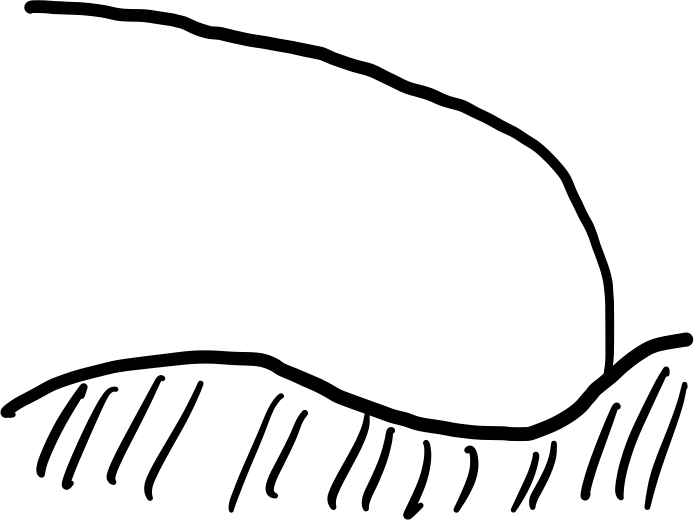
\includegraphics[width=30mm]{figs/unbounded.png}} node[xshift=-2mm, yshift=1mm] at (unbounded.center) {{\small \emph{ice}}};
  \node[right=of unbounded] (wedge) {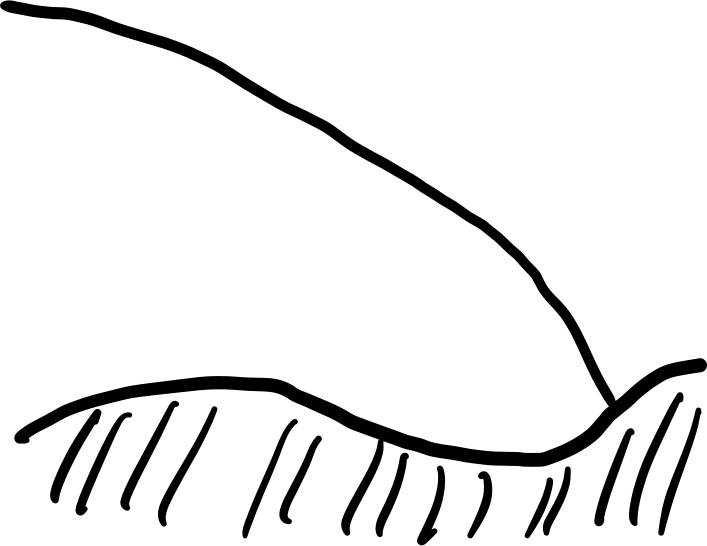
\includegraphics[width=30mm]{figs/wedge.png}} node[xshift=-4mm, yshift=1mm] at (wedge.center) {{\small \emph{ice}}};
  \node[right=of wedge] (realistic) {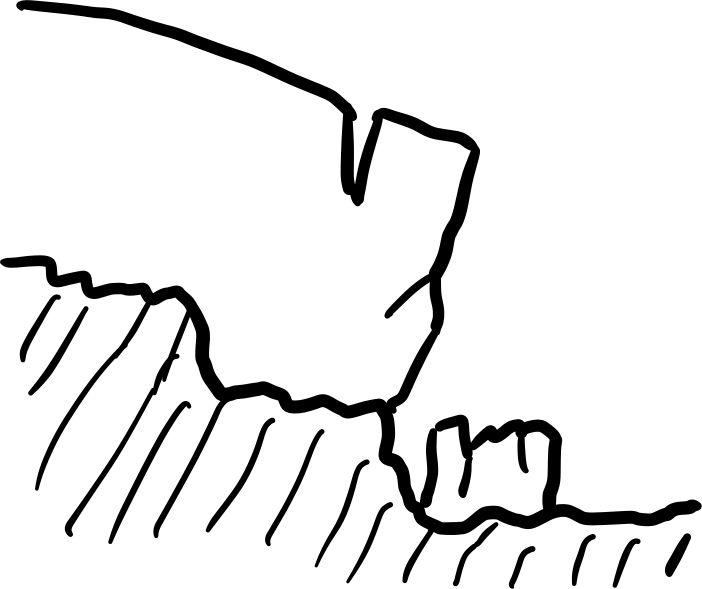
\includegraphics[width=30mm]{figs/realistic.png}} node[xshift=-6mm, yshift=4mm] at (realistic.center) {{\small \emph{ice}}};
\end{tikzpicture}
\end{center}

\vspace{-2mm}

\caption{In which Sobolev space should we seek the surface elevation function?  This question relates to the expected shapes of ice margins.  The shallow ice theory yields fractional power shapes (left), but other models suggest a finite-slope ``wedge'' shape (center).  Actual glacier margins often have overhangs, crevasses, and cliffs (right).}
\label{fig:margins}
\end{figure}

Reality is of course more complicated.  In the vicinity of an ice margin, especially on steep bedrock features, real glacier ice can generate overhangs which violate the assumption of a single-valued surface elevation function, and even the bedrock can overhang.  Fractures, crevasses, and cliffs are also commonly found in glacier margins, but modeling such features would depart from our viscous fluid paradigm.  In fact, because margins are small features compared to the overall scale of glaciers and ice sheets, most modeling literature ignores overhangs and assumes instead that surface and bed elevation functions are well-defined; see \cite{IsaacStadlerGhattas2015,Jouvetetal2008,LofgrenAhlkronaHelanow2022,WirbelJarosch2020} among many examples.

Making progress on this situation might require extending the Stokes-based viscous models considered here by allowing fractures, for example by supplementing momentum conservation with an additional advected damage variable \cite{PralongFunk2005}, such that ice-cliff calving occurs via a stress-failure criterion.  The resulting emergent margin shapes might suggest an appropriate regularity assumption, i.e.~Sobolev space, for surface elevations, within a viscous-only theory.

\subsection{On the convergence of explicit time-stepping} \label{subsec:explicit}  This paper makes some progress toward a convergence theorem for a fully-discrete scheme applied to the space-time problem \eqref{eq:icydomain}--\eqref{eq:stokes}.  Our strategy considers the implicitly time-discretized, but spatially continuous, VI problem \eqref{eq:be:vi}.  Looking ahead, Theorem \ref{thm:glacierapp} will bound the numerical error in an FE scheme for that implicit-step problem.  However, we will neither address well-posedness of the continuous space-time problem, nor bound errors made by a fully-discrete scheme.

To put this approach in context one might consider the explicit time-stepping alternative.  First consider a glacier that does not flow.  Time-step problem \eqref{eq:be:vi} then reduces to determining the geometry according only to the SMB and the prior geometry, a problem which turns out to be well-posed over $L^2(\Omega)$.  To see this precisely, let $F^{\bzero}_{\Delta t}(s)[q] = \int_\Omega sq$, which sets $\bu|_s=\bzero$ in \eqref{eq:be:Fdefine}.  Assuming that definition \eqref{eq:be:source} yields $\ell^n \in L^2(\Omega)$, there exists a unique solution $s \in \cK_{L^2} = \left\{r\in L^2(\Omega)\,:\,r \ge b\right\}$ of the no-flow VI problem
\begin{equation}
F^{\bzero}_{\Delta t}(s)[r-s] \ge \ell^n[r-s] \quad \text{for all } r \in \cK_{L^2}, \label{eq:explicit:noflow}
\end{equation}
which is given by truncation \cite[section II.3]{KinderlehrerStampacchia1980}:
\begin{equation}
s = \max\{b, \ell^n\} = \max\{b, s^{n-1} + \Delta t\,a^n\} \qquad (\text{\emph{no flow}}).
\end{equation}
Thus, in the absence of flow, the new surface can be (explicitly) raised or lowered according to the (pointwise) integral of the SMB rate, then truncated so that it does not go below the bed.  This is obvious, and not usually stated in such mathematical terms.

However, an explicit time-step of the real glacier geometry problem has the same mathematical character as in the no-flow problem \eqref{eq:explicit:noflow}.  Suppose $s^{n-1}$ is admissible and sufficiently regular so that $\bn_{s^{n-1}}$ is well-defined, and so that the weak-form Stokes problem \eqref{eq:glenstokes:weak} is well-posed over the domain $\Lambda_{s^{n-1}}$.  The explicit operator
\begin{equation}
F^{\text{e}}_{\Delta t}(s)[q] = \int_\Omega \left(s - \Delta t\, \bu|_{s^{n-1}} \cdot \bn_{s^{n-1}}\right) q  \label{eq:explicitFdefine}
\end{equation}
then arises by applying forward Euler to SKE \eqref{eq:ske}; compare definition \eqref{eq:be:Fdefine}.  The explicit VI problem corresponding to \eqref{eq:be:vi}, namely
\begin{equation}
F^{\text{e}}_{\Delta t}(s)[r-s] \ge \ell^n[r-s] \quad \text{for all } r \in \cK_{L^2}, \label{eq:explicit:vi}
\end{equation}
is again well-posed, and again it can be solved for $s \in \cK_{L^2}$ by truncation:
\begin{equation}
s = \max\{b, s^{n-1} + \Delta t\, \bu|_{s^{n-1}} \cdot \bn_{s^{n-1}} + \Delta t\,a^n\} \qquad (\text{\emph{explicit step}}). \label{eq:explicit:solution}
\end{equation}

Now consider a fully-discrete forward Euler scheme wherein an FE approximation of VI problem \eqref{eq:explicit:vi} is computed at each time step.  Such a scheme\footnote{Explicit schemes like this have practical value.  For example, Equation \eqref{eq:explicit:solution} is precisely the approach in \cite{Lengetal2012}, for example, and \cite{Jouvetetal2008} is likewise explicit.  Various semi-implicit modifications have also been used \cite{Chengetal2020,Durandetal2009,LofgrenAhlkronaHelanow2022,WirbelJarosch2020}.} computes an FE approximation of the exact solution \eqref{eq:explicit:solution}.  However, in formula \eqref{eq:explicit:solution} the derivatives in $\bn_{s^{n-1}}$, the trace evaluation $\bu|_{s^{n-1}}$, and the truncation itself all (generally) reduce regularity of $s$  relative to $s^{n-1}$.  From what we know about well-posed Stokes problems, the function $s$ defined by \eqref{eq:explicit:solution} generally will not be regular enough, i.e.~sufficiently differentiable in space, to serve as the surface elevation at the start of the next time step.  That is, it is not clear that $s$ from \eqref{eq:explicit:solution} defines a sufficiently-smooth domain $\Lambda_s$ so that the (weak) Stokes problem \eqref{eq:glenstokes:weak} is well-posed, that is, when we seek the next surface elevation $s^{n+1}$ after $s=s^n$.  In this sense there is no reason to expect the \emph{explicitly} time semi-discretized problems to be well-posed (after the first time step).

The regularity of the surface elevation solution might be improved by use of semi-implicit time-stepping, for example using $s$ in the surface normal in \eqref{eq:explicitFdefine}, $\bn_{s^{n-1}} \to \bn_s$, but leaving the old velocity in place.  However, \cite{LofgrenAhlkronaHelanow2022} demonstrate that this change, by itself, has small effect on stability, and it is not clear why it would suffice to address the regularity and well-posedness concerns.

None of this is to assert that a fully-discrete (space-time) scheme cannot converge to the continuum solution of the problem \eqref{eq:icydomain}--\eqref{eq:stokes}, or more precisely its
parabolic VI weak form \cite{Glowinski1984}.  (A proof of the well-posedness of the parabolic VI associated to strong form \eqref{eq:icydomain}--\eqref{eq:stokes} would be of great value here.)  However, as is well-understood in outline, but not settled quantitatively \cite{Chengetal2017}, convergence of an explicit scheme will be subject to a restriction on the (space-time) refinement path.  Besides being currently unclear (i.e.~in theory) what precisely is this restriction, the restriction will be worse than that for purely-advective problems, for the reasons already stated in Subsection \ref{subsec:notadv}, with corresponding negative effects on numerical model performance \cite{Bueler2023}.

\subsection{Conjectural well-posedness for the implicit time-step problem} \label{subsec:conjecture} Subsections \ref{subsec:notadv}--\ref{subsec:explicit} have deployed various imperfect arguments to explain why the backward Euler VI problem \eqref{eq:be:vi} could be well-posed, or at least why other approaches are less promising.  We now state a mathematically-precise conjectural framework for well-posedness of this problem based upon the idea that the surface motion map $\Phi(s) = -\bu|_s\cdot \bn_s$ assigns different values to inputs which differ in Sobolev norm, and that it does so in a controlled and positive-definite manner.

\begin{conjecture}[Surface motion $\Phi(s)$ is $\qq$-coercive over admissible surface elevations] \label{conj:b}  For $\rr>2$ such that Conjecture \ref{conj:a} holds, let $\cX = W^{1,\rr}(\Omega)$.  Fix $b\in\cX$ and let $\cK=\{r\in\cX\,:\,r|_{\partial\Omega}=b|_{\partial\Omega} \text{ and } r\ge b\}$.  Recall that $\Phi:\cK\to\cX'$ is then well-defined by Lemma \ref{lem:philipschitz}.  Then there are constants $\alpha>0$ and $\qq>1$ so that
\begin{equation}
\left(\Phi(r) - \Phi(s)\right)[r-s] \ge \alpha \|r-s\|_{\cX}^\qq \qquad \text{for all } r,s\in\cK. \label{eq:conj:b}
\end{equation}
\end{conjecture}

Inequality \eqref{eq:conj:b} is called $\qq$-\emph{coercivity} of $\Phi$ over $\cK$.  If an operator is both continuous and $\qq$-coercive, over a closed and convex subset of a Banach space, then the corresponding VI problem is well-posed (Section \ref{sec:abstractestimate}).  We prove next that Conjectures \ref{conj:a} and \ref{conj:b} together are sufficient for well-posedness of VI problem \eqref{eq:be:vi}.

\begin{theorem} \label{thm:stepwellposed}  Assume Conjectures \ref{conj:a} and \ref{conj:b}, and fix $b \in \cX$ to define $\cK$.  Suppose that $s^{n-1}\in\cK$, and that the SMB function $a=a(t,x)$ is in $C([0,T]; L^{\rr'}(\Omega))$.  Then $F_{\Delta t}$ defined by \eqref{eq:be:Fdefine} is both continuous and $\qq$-coercive, and thus there exists a unique surface elevation $s\in\cK$ satisfying VI problem \eqref{eq:be:vi}. \end{theorem}

\begin{proof}  Let $R>0$.  By Lemma \ref{lem:philipschitz} there is $C(R)>0$ so that if $r,s\in B_R\cap\cK$ then $\big|\Phi(r)[q] - \Phi(s)[q]\big| \le C(R) \|r-s\|_{\cX} \|q\|_{\cX}$.  Then by definition \eqref{eq:be:Fdefine}, H\"older's inequality, and Sobolev's inequality we have
\begin{align}
\left|F_{\Delta t}(r)[q] - F_{\Delta t}(s)[q]\right| &\le \int_\Omega |r-s||q| + \Delta t\, \big|\Phi(r)[q] - \Phi(s)[q]\big| \\
    &\le C \|r-s\|_{\cX} \|q\|_\cX \notag
\end{align}
for some $C>0$ which depends on $R$ and $\Delta t$.  Thus $F_{\Delta t}$ is (Lipschitz) continuous on bounded subsets of $\cK$.  If Conjecture \ref{conj:b} holds then
\begin{align}
\left(F_{\Delta t}(r) - F_{\Delta t}(s)\right)[r-s] &= \int_\Omega (r-s)^2 + \Delta t\, \left(\Phi(r) - \Phi(s)\right)[r-s] \\
    &\ge \alpha\Delta t \|r-s\|_{\cX}^\qq, \notag
\end{align}
so $F_{\Delta t}$ is $\qq$-coercive over $\cK$ with constant $\alpha\Delta t>0$.  From definition \eqref{eq:be:source}, the hypothesis on $a$, and H\"older's inequality,
\begin{equation}
\big|\ell^n[q]\big| \le \left(\|s^{n-1}\|_{L^{\rr'}} + \Delta t \max_{t\in[t_{n-1},t_n]} \|a(t,\cdot)\|_{L^{\rr'}}\right) \|q\|_{L^\rr}
\label{eq:sourcetermbound}
\end{equation}
for all $q \in \cX$.  Because $\|s^{n-1}\|_{L^{\rr'}}<\infty$ by Sobolev's inequality, and $\|q\|_{L^\rr} \le \|q\|_{\cX}$, it follows that $\ell^n \in \cX'$.  Because $F_{\Delta t}$ is $\qq$-coercive it is also coercive and strictly-monotone (Definition \ref{def:monotonecoercive}).  Now Corollary III.1.8 of \cite{KinderlehrerStampacchia1980} shows unique existence of a solution to \eqref{eq:be:vi}.
\end{proof}

Theorem \ref{thm:stepwellposed} addresses only the well-posedness of a single time-step problem over $[t_{n-1},t_n]$.  Its conclusion is not sufficient to show well-posedness of the time-dependent problem parabolic VI problem over $[0,T]$ corresponding to NCP \eqref{eq:ncp}.  If this problem were known to be well-posed then one might analyze whether implicit steps converge in the $\Delta t\to 0$ limit.

The two Conjectures may be difficult to prove despite some progress in Sections \ref{sec:stokes} and \ref{sec:model}.  Greater progress has been made in the SIA case \cite{Calvoetal2003,JouvetBueler2012,PiersantiTemam2023}, which could be helpful.  In any case, the computation of $\bu|_s$ and $\Phi(s)=-\bu|_s\cdot \bn_s$, or equivalent expressions, is necessary in any evolving-geometry Stokes framework, implicit or not, and modeling practitioners apparently expect such expressions to be well-behaved in some manner.


\section{Numerical exploration of \texorpdfstring{$2$}{2}-coercivity} \label{sec:numerical}

We may explore the validity of Conjecture \ref{conj:b} by sampling from numerical simulations.  The experiments here,\footnote{Source code is at the public repository \href{https://github.com/bueler/glacier-fe-estimate}{\texttt{github.com/bueler/glacier-fe-estimate}}, in the \texttt{py/} directory.  The codes call the library at \href{https://github.com/bueler/stokes-extrude}{\texttt{github.com/bueler/stokes-extrude}}.} performed using Python and the Firedrake FE library \cite{Hametal2023}, are not intended to demonstrate implicit time-stepping, but only to generate admissible surface elevation pairs $r,s\in\cK$ to use as samples.  For a given sample pair we evaluate the $2$-coercivity ratio
\begin{equation}
\rho(r,s) = \frac{\left(\Phi(r) - \Phi(s)\right)[r-s]}{\|r-s\|_{\cX}^2}. \label{eq:Phiratio}
\end{equation}
If, for all pairs in some $\cK$, the set of ratios $\{\rho(r,s)\}$ were bounded below by a positive constant $\alpha>0$, then this would confirm the $\qq=2$ coercivity inequality \eqref{eq:conj:b} for that $\cK$.  Of course, a numerical experiment allows only finite sampling, and furthermore a finite spatial discretization must be used.

The domain for our experiments is the 1D interval $\Omega=(-L,L)$, $L=100$ km, with $\cX = W_b^{1,2}(\Omega)$.  The interval $\Omega$ was uniformly-meshed into equal intervals.  The $P_1$ piecewise-linear FE space $\cX_h\subset \cX$ was used for the bed $b$ and the surface $s$, giving polygonal domains $\Lambda$ defined by $b,s$; see equation \eqref{eq:icydomain}.  Three bed profiles  (Figure \ref{fig:cases}) were considered, \emph{flat} with $b=0$, \emph{smooth} with a superposition of several wavelengths down to 10 km, and \emph{rough} with an additional 4 km wavelength mode.  These beds generate corresponding constraint sets $\cK_i \subset \cX$, $i=1,2,3$.

\begin{figure}[ht]
\mbox{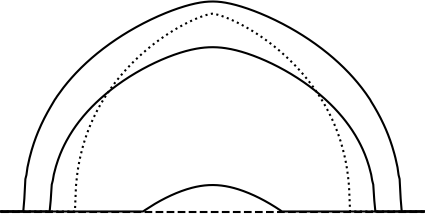
\includegraphics[width=0.30\textwidth]{figs/snapsflat.png} \, 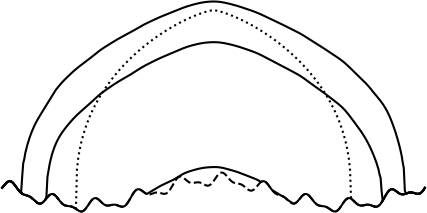
\includegraphics[width=0.32\textwidth]{figs/snapssmooth.png} \, 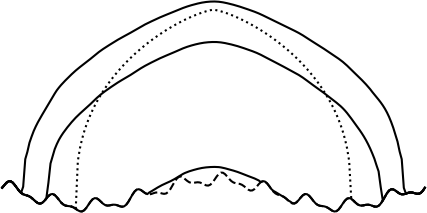
\includegraphics[width=0.32\textwidth]{figs/snapsrough.png}}

\caption{Three bed cases (flat, smooth, rough) define constraint sets $\cK_i\subset\cX$ in the numerical experiment.  For each $\cK_i$, three time-dependent runs of $T=200$ years, starting from the same initial state (dotted), but using different constant values of the SMB (see text), generated a large number of admissible states.  Example states at $t=170$ years are shown (solid).  Ratios \eqref{eq:Phiratio} were computed for 1000 sample pairs $r,s$ from each set $\cK_i$.}
\label{fig:cases}
\end{figure}

For each constraint set $\cK_i$, three constant SMB values were considered (units $\text{m}\,\text{s}^{-1}$): $a=\{-2.5,0.0,1.0\}\times 10^{-7}$.  For each SMB value a time-dependent run of duration $T=200$ years started from the same initial surface elevation profile.\footnote{A Halfar profile \cite{Halfar1981} with characteristic time $t_0=29$ years was used as the initial state.  In the case of a flat bed and $a=0$ the exact time-dependent solution under SIA dynamics is known by Halfar's result \cite{Halfar1981}.  The final ($T=200$ a) surface elevation, from using Stokes dynamics in the actual experiment, agrees closely with the SIA exact solution; compare comments in \cite{LofgrenAhlkronaHelanow2022}.}  The positive SMB value was sufficient to advance the ice margins nearly to the domain boundary at $|x|=L$ by the final time $T$, while the negative SMB value caused the glacier to disappear entirely by that time.

In these simulations each time-step VI \eqref{eq:be:vi} was done semi-implicitly.  That is, definition \eqref{eq:be:Fdefine} was modified to use the prior surface velocity $\bu|_{s^{n-1}}$.  The numerical VI solution was by a reduced-space Newton method with line search \cite{BensonMunson2006}.  The ``FSSA'' stabilization technique from \cite{LofgrenAhlkronaHelanow2022} was applied, which generates a modified Stokes weak form compared to \eqref{eq:glenstokes:weak}; see equation (23) in \cite{LofgrenAhlkronaHelanow2022}.  The Stokes problem \eqref{eq:glenstokes:weak}, with viscosity regularization $\eps=10^{-19}\, \text{s}^{-2}$ in \eqref{eq:glen}, was solved on each domain $\Lambda$ using a vertically-extruded mesh of quadrilaterals (Figure \ref{fig:fe:operatorvisualization}), mixed FE method for the $Q_2\times Q_1$ (Taylor-Hood) stable pair \cite{Elmanetal2014}, and a Newton solver, with direct solution of the linear step equations.  The resulting time-dependent numerical method is only conditionally stable, but adequate for our purpose of generating sample surfaces.

The basic result of these experiments is shown in Figure \ref{fig:ratios}.  These are sample ratio $\rho(r,s)$ histograms from the highest spatial resolution, namely $\Delta x=500$ m and 40 elements in each extruded column.  More than $87\%$ of all the ratios were positive, and of these the medians for the three $\cK_i$ were in the range $[4.5,5.2] \times 10^{-13}$.  For the remaining negative ratios, the medians were in the range $[-4.1,-2.8]\times 10^{-14}$, much smaller in magnitude.

\begin{figure}[ht]
\mbox{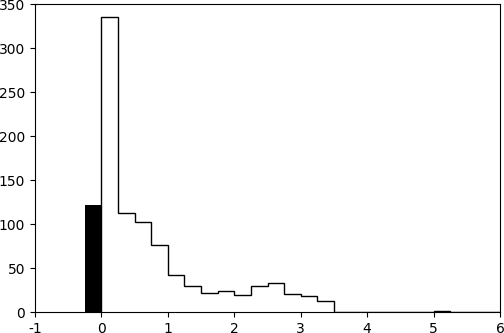
\includegraphics[width=0.32\textwidth]{figs/flatratios.png} \, 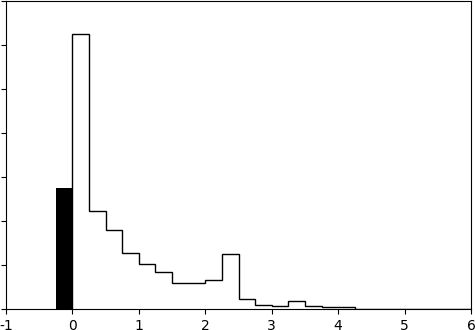
\includegraphics[width=0.30\textwidth]{figs/smoothratios.png} \, 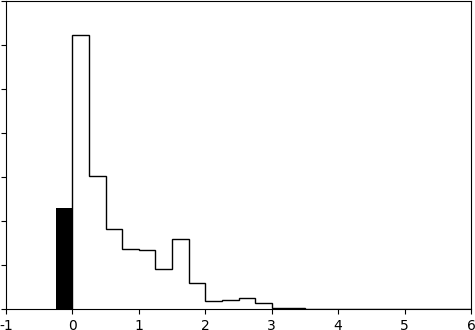
\includegraphics[width=0.30\textwidth]{figs/roughratios.png}}

\caption{Histograms of ratios $\rho(r,s)$ for 1000 sample pairs from each of the three sets $\cK_i$ (Figure \ref{fig:cases}).  The horizontal axis has  $\rho(r,s) \in [-1,6]\times 10^{-12}$, and the common vertical axis is for counts between 0 and 350.  About $10\%$ of these ratios are negative (solid).}
\label{fig:ratios}
\end{figure}

Figure \ref{fig:ratios} does \emph{not} represent compelling evidence of $2$-coercivity by definition \eqref{eq:qcoercive}, but it does not exclude it.  In fact, the details of the discretization of the ice margin strongly influence the negative ratios.  Noting that ratio evaluation uses integral \eqref{eq:definePhi}, if that integrand is reset to zero where the ice is thinner than 100 m then the negative values disappear (not shown).  Even without such thresholding, at lower horizontal resolution ($\Delta x=2000$ m) the median magnitude of negative ratios was roughly twice as large (not shown).  The disappearance of negative ratios under grid refinement therefore should not be excluded.  Margin approximation improvements, such as adaptive/local mesh refinement, will probably improve the numerical evidence for $2$-coercivity.

It is theoretically possible that the operator $\Phi$ is monotone---see inequality \eqref{eq:monotone}---but not $\qq$-coercive for any $\qq$.  In that case a revised well-posedness argument can be attempted, for example by adding a small coercive form as in section III.2 of \cite{KinderlehrerStampacchia1980}.  However, if a continuum pair $r,s$ with a negative ratio were actually to be found in some $\cK$, i.e.~with an exact continuum ratio $\rho(r,s)<0$ from \eqref{eq:Phiratio}, then the coercivity-based well-posedness framework of this paper would fail unless VI problem \eqref{eq:be:vi} is permanently regularized.

Regarding Conjecture \ref{conj:a}, i.e.~Lipschitz continuity for the surface velocity trace, the ratio $\big\|\bu|_r - \bu|_s\big\|_{L^2}/\|r-s\|_{W^{1,2}}$ for the same sample pairs was also evaluated.  Over all three sets $\cK_i$, at the highest resolution, the maximum ratio was $3.5\times 10^{-9}$, providing a lower bound for $C_A$.  Again, numerical experiments obviously cannot prove Conjecture \ref{conj:a}.


\section{Abstract error estimate for finite element approximation of VIs} \label{sec:abstractestimate}

In this Section we consider the FE approximation of an abstract VI problem.  We will return to glaciological problem \eqref{eq:be:vi} in Section \ref{sec:application}.

Let $\cX$ be a real reflexive Banach space with norm $\|\cdot\|$ and topological dual (Banach) space $\cX'$.  Denote the dual pairing of $\ell \in \cX'$ and $v\in\cX$ by $\ell[v]$, and define $\|\ell\|_{\cX'} = \sup_{\|v\|=1} \big|\ell[v]\big|$.  Let $\cK \subset \cX$ be a nonempty, closed, and convex subset, called the constraint set, whose elements are called admissible.  For a continuous, but generally nonlinear, operator $f:\cK \to \cX'$, and a source functional $\ell\in \cX'$, the VI problem is to find $u\in \cK$ such that
\begin{equation}
f(u)[v-u] \ge \ell[v-u] \quad \text{for all } v\in \cK. \label{eq:vi}
\end{equation}
VI problem \eqref{eq:be:vi} is in this form, but the best known example is the obstacle problem for the Laplacian operator---see \cite{Ciarlet2002,Evans2010,KinderlehrerStampacchia1980} for theory and FE analysis.  A key observation is that $f(u)-\ell \in \cX'$ is generally nonzero when $u$ solves \eqref{eq:vi}, though if $u$ is in the interior of $\cK$ then $f(u)=\ell$.  Under sufficient regularity assumptions an NCP like \eqref{eq:ncp} or \eqref{eq:be:ncp} follows from \eqref{eq:vi}.

\begin{definition} \label{def:monotonecoercive}
An operator $f:\cK \to \cX'$ is said to be \emph{monotone} if
\begin{equation}
\left(f(v)-f(w)\right)[v-w] \ge 0 \qquad \text{for all } v,w \in \cK \label{eq:monotone}
\end{equation}
and \emph{strictly monotone} if equality in \eqref{eq:monotone} implies $v=w$ \cite{Minty1963}, \cite[Chapter III]{KinderlehrerStampacchia1980}.  It is \emph{coercive} if there is $w\in \cK$ so that $\left(f(v)-f(w)\right)[v-w]/\|v-w\| \to +\infty$ for $v \in \cK$ as $\|v\| \to +\infty$.  It is \emph{$\qq$-coercive} \cite{Bueler2021conservation}, for some $\qq>1$, if there exists $\alpha>0$ such that
\begin{equation}
\left(f(v)-f(w)\right)[v-w] \ge \alpha \|v-w\|^\qq \qquad \text{for all } v,w \in \cK. \label{eq:qcoercive}
\end{equation}
(The definition of $\qq$-coercive was already given in Conjecture \ref{conj:b}.)
\end{definition}

If $f:\cK \to \cX'$ is monotone and coercive, and also continuous on finite-dimensional subspaces, then VI \eqref{eq:vi} has a solution \cite[Corollary III.1.8]{KinderlehrerStampacchia1980}.  If $f$ is strictly monotone then the solution is unique.  If $f$ is $\qq$-coercive then it coercive and strictly monotone, so $\qq$-coercivity and continuity yield well-posedness for \eqref{eq:vi}.  Note that Definitions \ref{def:monotonecoercive} and \ref{def:lipshitz} do not require $f$ to be defined on all of $\cX$, but only on $\cK$.
  
The following definition appeared in Lemma \ref{lem:philipschitz}.  If it holds then $f$ is continuous.

\begin{definition} \label{def:lipshitz}
For $R>0$ let $B_R = \{v\in \cX\,:\,\|v\|\le R\}$.  We say $f:\cK \to \cX'$ is \emph{Lipshitz on bounded subsets of $\cK$} if for every $R>0$ there is $C(R)>0$ so that if $v,w \in B_R \cap \cK$ and $z\in\cX$ then $|\left(f(v)-f(w)\right)[z]| \le C(R) \|v-w\| \|z\|$, equivalently
\begin{equation}
\|f(v)-f(w)\|_{\cX'} \le C(R) \|v-w\| \quad \text{ for all } v,w \in B_R \cap \cK.  \label{eq:liponbounded}
\end{equation}
\end{definition}

An FE method for \eqref{eq:vi} becomes a finite-dimensional VI problem.  Suppose $\cX_h \subset \cX$ is a finite-dimensional subspace, typically some space of continuous, piecewise-polynomial functions defined on a mesh.  The FE constraint set $\cK_h\subset \cX_h$ is assumed to be closed and convex, but generally $\cK_h \nsubseteq \cK$.  Let $f_h:\cK_h\to\cX'$, and note that generally $f_h\ne f$ because of quadrature and other approximations.  (Looking ahead to Section \ref{sec:application}, both $\cK_h \nsubseteq \cK$ and $f_h\ne f$ occur naturally in the glacier geometry problem.)  The FE VI problem is
\begin{equation}
f_h(u_h)[v_h-u_h] \ge \ell[v_h-u_h] \quad \text{for all } v_h\in \cK_h. \label{eq:fe:vi}
\end{equation}
We will assume that \eqref{eq:fe:vi} has a solution $u_h\in\cK_h$.

The following FE error estimation theorem extends the well-known result by Falk \cite{Falk1974}.  See also Theorem 5.1.1 in \cite{Ciarlet2002}, and the version of the estimate wherein $u$ (but not $u_h$) solves a variational \emph{equality} in \cite[Theorem 1]{KirbyShapero2024}.  For the proof we must assume that the domain of $f$ includes the FE solution, which is achieved here by defining a convex superset of $\cK$ and $\cK_h$.  This technical assumption permits a clean and general estimation theorem, but the choice of $\cK_h$ made in Section \ref{sec:application} means that the convex hull construction is not needed in our glacier application; see also Corollary \ref{cor:abstractestimate:nohull}.

\begin{theorem} \label{thm:abstractestimate}  Let $\hcK$ be the closure in $\cX$ of the convex hull of $\cK \cup \cK_h$, and suppose that $f:\hcK \to \cX'$.  For $\qq>1$, with conjugate exponent $\qq'=\qq/(\qq-1)$, assume that $f$ is $\qq$-coercive over $\hcK$ with constant $\alpha>0$, and Lipshitz on bounded sets of $\hcK$.  Suppose $u\in\cK$ solves \eqref{eq:vi} and $u_h\in\cK_h$ solves \eqref{eq:fe:vi}, and let $R_h=\max\{\|u\|,\|u_h\|\}$.  Then there is a constant $c=c(R_h,\alpha)>0$, not otherwise depending on $u$ or $u_h$, so that
\begin{align}
\|u-u_h\|^\qq &\le \quad \frac{2}{\alpha} \inf_{v\in\cK} \left(f(u)-\ell\right)[v-u_h] \label{eq:abstractestimate} \\
   &\quad\, + \frac{2}{\alpha} \inf_{v_h\in\cK_h} \left(f(u)-\ell\right)[v_h-u] \notag \\
   &\quad\, + \frac{2}{\alpha} \left(f(u_h)-f_h(u_h)\right)[u_h] \notag \\
   &\quad\, + c \inf_{v_h\in\cK_h} \|v_h - u\|^{\qq'}. \notag
\end{align}
\end{theorem}

\begin{proof}  For arbitrary $v\in\cK$ and $v_h\in\cK_h$, rewrite \eqref{eq:vi} and \eqref{eq:fe:vi} as follows:
\begin{align}
f(u)[u]     &\le f(u)[v] + \ell[u-v], \label{eq:abstract:one}  \\
f_h(u_h)[u_h] &\le f_h(u_h)[v_h] + \ell[u_h-v_h]. \notag
\end{align}
It follows from \eqref{eq:abstract:one} and $\qq$-coercivity of $f$ that
\begin{align}
\alpha \|u-u_h\|^\qq &\le \left(f(u)-f(u_h)\right)[u-u_h] \label{eq:abstract:two} \\
  &= f(u)[u] + f(u_h)[u_h] - f(u)[u_h] - f(u_h)[u] \notag \\
  &= f(u)[u] + f_h(u_h)[u_h] \notag \\
  &\qquad - f(u)[u_h] - f(u_h)[u] + \left(f(u_h)-f_h(u_h)\right)[u_h] \notag \\
  &\le f(u)[v] + \ell[u-v] + f(u_h)[v_h] + \ell[u_h-v_h] \notag \\
  &\qquad - f(u)[u_h] - f(u_h)[u] + \left(f(u_h)-f_h(u_h)\right)[u_h] \notag \\
  &= f(u)[v-u_h] - \ell[v-u_h] + f(u_h)[v_h-u] - \ell[v_h-u] \notag \\
  &\qquad + \left(f(u_h)-f_h(u_h)\right)[u_h] \notag \\
  &= \left(f(u)-\ell\right)[v-u_h] + \left(f(u)-\ell\right)[v_h-u] \notag \\
  &\qquad + \left(f(u)-f(u_h)\right)[u-v_h] + \left(f(u_h)-f_h(u_h)\right)[u_h] \notag
\end{align}
Since $u,u_h\in B_{R_h}$, by the Lipshitz assumption over $\hcK$ there is $C(R_h)>0$ so that
\begin{equation}
\left(f(u)-f(u_h)\right)[u-v_h] \le C(R_h) \|u-u_h\|\|u-v_h\|. \label{eq:abstract:three}
\end{equation}
Noting $1<\qq<\infty$, now use Young's inequality with $\eps>0$ \cite[Appendix B.2]{Evans2010}:
\begin{align}
\alpha \|u-u_h\|^\qq &\le \left(f(u)-\ell\right)[v-u_h] + \left(f(u)-\ell\right)[v_h-u]  \label{eq:abstract:four} \\
  &\qquad + C(R_h) \left(\eps\|u-u_h\|^\qq + \tilde C(\eps) \|u-v_h\|^{\qq'}\right) \notag \\
  &\qquad + \left(f(u_h)-f_h(u_h)\right)[u_h], \notag
\end{align}
where $\tilde C(\eps) = (\eps \qq)^{-\qq'/\qq} {\qq'}^{-1}$.  Choose $\eps>0$ so that $C(R_h) \eps \le \alpha/2$, and subtract:
\begin{align}
\frac{\alpha}{2} \|u-u_h\|^\qq &\le \left(f(u)-\ell\right)[v-u_h] + \left(f(u)-\ell\right)[v_h-u]  \label{eq:abstract:five} \\
  &\qquad + C(R_h) \tilde C(\eps) \|u-v_h\|^{\qq'} + \left(f(u_h)-f_h(u_h)\right)[u_h] \notag
\end{align}
Take infimums to show \eqref{eq:abstractestimate}, and note that $c=2 C(R_h) \tilde C(\eps)/\alpha$.
\end{proof}

Note that Theorem \ref{thm:abstractestimate} does \emph{not} assume any of the following: $\cK_h \subset \cK$, $f$ is linear, $f_h=f$, $f_h$ is continuous, or $f_h$ is $\qq$-coercive.  We also do not require that $u_h$ is the \emph{unique} solution of \eqref{eq:fe:vi}; the result holds for any solution.

The next Corollary, the proof of which is immediate, addresses two important cases where the convex hull operation is not needed.  We will see in Section \ref{sec:application} that case \emph{i)} can be chosen within a glacier simulation.

\begin{corollary}  \label{cor:abstractestimate:nohull}  Suppose that one of the following situations apply:
\renewcommand{\labelenumi}{\roman{enumi})}
\begin{enumerate}
\item $\cK_h \subset \cK$, or
\item $f$ is defined on all of $\cX$.
\end{enumerate}
Assume $f$ is $\qq$-coercive on, and Lipschitz on bounded subsets of, its domain, namely $\cK$ or $\cX$, respectively.  Otherwise make the assumptions of Theorem \ref{thm:abstractestimate}.  Then conclusion \eqref{eq:abstractestimate} holds.  Additionally, in case i) the ``\,$\inf_{v\in\cK}$'' term is zero.
\end{corollary}

Consider $f(u)-\ell\in \cX'$.  It might be a measure or a measurable function, and then the first two terms in estimate \eqref{eq:abstractestimate} use information about its support.  (This plays a role in the glacier application of Section \ref{sec:application}.)  By contrast, the original Hilbert space result by Falk \cite{Falk1974} computes norms and loses this information.  The following Corollary, with easy proof, mimics this norm-based approach.  We suppose that $\cX$ continuously and densely embeds into a larger Banach space $\cB$:
\begin{equation}
\cX \hookrightarrow \cB, \quad \bar{\cX} = \cB \label{eq:VembedsinB}
\end{equation}
Observe that \eqref{eq:VembedsinB} implies $\cB' \subset \cX'$.  A standard example is $\cX=W^{1,\rr}(\Omega)$ and $\cB=L^\rr(\Omega)$.

\begin{corollary}  \label{cor:abstractestimate:Bnorm}  In addition to the assumptions of Theorem \ref{thm:abstractestimate}, suppose \eqref{eq:VembedsinB} holds, and that $\|f(u)-\ell\|_{\cB'} < \infty$.  Then
\begin{align}
\|u-u_h\|^\qq &\le \frac{2}{\alpha} \|f(u)-\ell\|_{\cB'} \left( \inf_{v\in\cK} \|v-u_h\|_{\cB} +   \inf_{v_h\in\cK_h} \|v_h-u\|_{\cB} \right) \label{eq:abstractestimate:Bnorm} \\
   &\qquad + \frac{2}{\alpha} \left(f(u_h)-f_h(u_h)\right)[u_h] + \inf_{v_h\in\cK_h} c \|v_h - u\|^{\qq'} \notag
\end{align}
\end{corollary}

The result in \cite{Falk1974} can be recovered by combining the above two Corollaries, with the further assumptions that $f$ is linear and $f_h=f$.  To say this precisely, suppose $f(v)[w]=a(v,w)$ is bilinear, uniformly elliptic, and continuous on a Hilbert space $\cX$.  The definition of uniformly elliptic then coincides with definition \eqref{eq:qcoercive} of $2$-coercive, and continuity of $a(v,w)$ implies \eqref{eq:liponbounded}.  Suppose that $\cX\hookrightarrow \cH$ and $\bar{\cX} = \cH$ for some Hilbert space $\cH$, and that $\|f(u)-\ell\|_{\cH'} < \infty$ so that, up to isomorphism, $f(u)-\ell \in \cH$.  Finally, suppose that $f(u_h)=f_h(u_h)$.  Then case \emph{ii)} of Corollary \ref{cor:abstractestimate:nohull} combines with Corollary \ref{cor:abstractestimate:Bnorm} to yield Theorem 1 in \cite{Falk1974}.

The ``$\inf_{v\in\cK}$'' term in estimates \eqref{eq:abstractestimate} and \eqref{eq:abstractestimate:Bnorm} is generally nonzero in obstacle problems where $\cK_h \not\subset \cK$.  To see how this case can occur, consider a unilateral obstacle problem where $\cK=\{v \in \cX\,:\,v\ge \psi\}$.  Suppose $\psi_h=\pi_h \psi$ is the FE interpolant of $\psi$, and define $\cK_h=\{v_h \in \cX_h\,:\,v_h\ge \psi_h\}$.  While $\psi_h(x_j)=\psi(x_j)$ for interpolation nodes $x_j$, generally $\psi_h(x) \ge \psi(x)$ will not hold for all $x\in\Omega$ even if $\psi$ is arbitrarily smooth, nor will $\psi_h(x) \le \psi(x)$ hold (Figure \ref{fig:nonadmissible}, left; see also \cite[Figure 5.1.3]{Ciarlet2002}).

\begin{figure}[ht]
\begin{center}
\begin{tikzpicture}[scale=1.1, domain=0.0:4.0, samples=200]
  \draw[black,thin,->] (-0.3,0.0) -- (4.5,0.0) node [xshift=2mm] {$x$};
  \draw plot (\x, {1.5 + 0.8 * cos(1.8*\x r)});
  \node[yshift=-2mm] at (2.0, 0.7) {$b$};
  \newcommand{\xlist}{0.0, 1.0, 1.4, 2.4, 3.0, 4.0}
  \foreach \x [remember=\x as \lastx] in \xlist {
      \draw (\x, 0.0) circle (1.5pt);
      \filldraw (\x, {1.5 + 0.8 * cos(1.8*\x r)}) circle (1.5pt);
      \draw[dashed] (\lastx, {1.5 + 0.8 * cos(1.8*\lastx r)}) -- (\x, {1.5 + 0.8 * cos(1.8*\x r)});
  }
  \node[yshift=3mm] at (3.0, 0.0) {$x_i$};
  \node[xshift=3mm, yshift=-7mm] at (0.0, 2.3) {$b_h$};
\end{tikzpicture}
 \quad \begin{tikzpicture}[scale=1.1, domain=0.0:4.0, samples=200]
  \draw[black,thin,->] (-0.3,0.0) -- (4.5,0.0) node [xshift=2mm] {$x$};
  \draw plot (\x, {1.5 + 0.8 * cos(1.8*\x r)});
  \newcommand{\xlist}{0.0, 1.0, 1.4, 2.4, 3.0, 4.0}
  \newcommand{\xymaxlist}{0.0/2.3, 1.0/2.3, 1.4/1.3182, 2.4/2.0078, 3.0/2.3, 4.0/2.3}
  \foreach \x/\y in \xymaxlist {
      \draw (\x, 0.0) circle (1.5pt);
      \filldraw (\x, \y) circle (1.5pt);
  }
  \node[yshift=3mm] at (3.0, 0.0) {$x_i$};
  \draw[dashed] (0.0,2.3) -- (1.0,2.3) -- (1.4,1.3182) -- (2.4,2.0078) -- (3.0,2.3) -- (4.0,2.3);
  \node[yshift=-2mm] at (2.0, 0.7) {$\psi$};
  \node[xshift=5mm, yshift=-3mm] at (1.0, 2.3) {$\psi_h$};
\end{tikzpicture}

\end{center}
\caption{Nodal admissibility does not imply admissibility.  Left: If $\psi_h=\pi_h\psi$ is the interpolant of $\psi$ then generally $\cK_h\subset\cK$ will not hold.  Right: Defining the FE obstacle by $\psi_h=R^{\oplus} \psi$, using monotone nodal operator \eqref{eq:monotoneop}, implies $\cK_h\subset\cK$ because $\psi_h\ge \psi$.}
\label{fig:nonadmissible}
\end{figure}

For such unilateral problems we may bypass the above issue by using a monotone nodal operator, defined as follows.  Assume $P_1$ elements and a continuous obstacle $\psi$.  For a given triangulation $\cT_h$ and node $x_i$ let $N_i$ be the closure of the union of elements adjacent to $x_i$.  Define
\begin{equation}
(R^{\oplus}\psi)(x_i) = \max_{x \in N_i} \psi(x). \label{eq:monotoneop}
\end{equation}
(Compare a multilevel version of $R^{\oplus}$ in \cite{BuelerFarrell2024}.)  Let $\psi_h$ be the unique $P_1$ function with nodal values $(R^{\oplus}\psi)(x_i)$, and write $\psi_h(x)=R^{\oplus} \psi(x)$.  Then $\psi_h(x)\ge \psi(x)$ for all $x\in \Omega$, so $\cK_h\subset \cK$ (Figure \ref{fig:nonadmissible}; right).  When we return to the surface elevation based glacier problem in Section \ref{sec:application} we will use this monotone operator on the bed elevation.  Note that models which solve for ice thickness using $P_1$ elements do not need this step; here $\cK = \{v\in\cX\,:\,v\ge 0\}$, so $\cK_h=\cK\cap\cX_h \subset \cK$ holds if $\cX_h$ is the $P_1$ space and $\cK_h$ is the set of $P_1$ functions with nonnegative nodal values.

The following Corollary collects some conclusions one might draw from making further assumptions.  Note that \eqref{eq:abstractestimate:subset:Cea} is Cea's lemma \cite[Theorem 2.4.1]{Ciarlet2002}, but in the Banach space $\cX$.  This PDE case, with no active set or free boundary, applies in the glacier context only when the entire domain $\Omega$ is covered in ice.

\begin{corollary}  \label{cor:abstractestimate:various}  Make the assumptions of case i) of Corollary \ref{cor:abstractestimate:nohull}.  Also assume that $f_h(u_h)[u_h] = f(u_h)[u_h]$.  Then
\begin{equation}
\|u-u_h\|^\qq \le  \inf_{v_h\in\cK_h} \left\{\frac{2}{\alpha} \left(f(u)-\ell\right)[v_h-u] + c \|v_h - u\|^{\qq'}\right\}. \label{eq:abstractestimate:subset}
\end{equation}
If also the assumptions of Corollary \ref{cor:abstractestimate:Bnorm} hold then
\begin{equation}
\|u-u_h\|^\qq \le \inf_{v_h\in\cK_h} \left\{\frac{2}{\alpha} \|f(u)-\ell\|_{\cB'} \|v_h-u\|_{\cB} + c \|v_h-u\|^{\qq'}\right\} \label{eq:abstractestimate:subset:Bnorm}
\end{equation}
If $f(u)=\ell$, for example if $u$ is in the interior of $\cK$, then
\begin{equation}
\|u-u_h\|^\qq \le c \inf_{v_h\in\cK_h} \|v_h-u\|^{\qq'} \label{eq:abstractestimate:subset:Cea}
\end{equation}
\end{corollary}


\section{Application to numerical glacier models} \label{sec:application}

Now we can synthesize the theory and apply it to an implicit time step of a Stokes-based glacier simulation.  This will give the phrase ``conforming FE method'' a precise meaning for such glacier simulations.  We will combine all previous threads: \emph{a)} well-posedness and \emph{a priori} bounds for the glaciological Stokes problem on a fixed domain (Section \ref{sec:stokes}), \emph{b)} conjectural well-posedness of the VI problem for an implicit time step of the surface elevation (Sections \ref{sec:model} and \ref{sec:theory}), and \emph{c)} the abstract error estimate for FE solutions of VIs (Section \ref{sec:abstractestimate}).

Consider an FE method for VI problem \eqref{eq:be:vi}, with $F_{\Delta t}$ defining in \eqref{eq:be:Fdefine}.  For a finite-dimensional subspace $\cX_h\subset \cX$, with a constraint set $\cK_h\subset \cX_h$, we seek $s_h\in\cK_h$ solving
\begin{equation}
F^h_{\Delta t}(s_h)[r_h-s_h] \ge \ell^n[r_h-s_h] \quad \text{for all } r_h \in \cK_h. \label{eq:fe:be:vi}
\end{equation}
The operator $F^h_{\Delta t}$ denotes an FE approximation to the operator $F_{\Delta t}$, but the source $\ell^n = s^{n-1} + \Delta t\,a^n$ is defined exactly as before, by equation \eqref{eq:be:source}.  We assume that the previous surface elevation $s^{n-1} \in \cK$ is general; we do not require $s^{n-1}\in\cK_h$.

Evaluation of $F^h_{\Delta t}(s_h)$ in the FE VI problem \eqref{eq:fe:be:vi} requires the nontrivial numerical solution of a glaciological Stokes problem \eqref{eq:glenstokes:weak} over a 3D mesh of the domain $\Lambda(s_h)$ between $z=b_h$ and $z=s_h$.  Solvability of this problem, for inf-sup stable elements, is addressed by \cite{Belenkietal2012,JouvetRappaz2011}.  The mesh need not be extruded vertically as shown in Figure \ref{fig:fe:operatorvisualization}, but this is a possibility.  However, the upper and lower surfaces, where boundary conditions \eqref{eq:stokes:stressfreesurface} and \eqref{eq:stokes:noslide} are applied, are assumed to be given by admissible FE functions, i.e.~$s_h,b_h\in\cX_h$ with $s_h\ge b_h$.  The numerical velocity from solving the Stokes problem, over the domain geometry defined by $s_h$, is denoted $\bu_h$, and its surface trace is denoted $\bu_h|_{s_h}$.  Observe that $\bu_h|_{s_h}$ will generally be different from the surface trace of the exact solution of the same Stokes boundary value problem for the same ($s_h$) geometry, denoted by $\bu|_{s_h}$.  Technically, the FE operator is defined as
\begin{equation}
F_{\Delta t}^h(s_h)[q] = \int_\Omega \left(s_h - \Delta t\, \bu_h|_{s_h}\cdot \bn_{s_h}\right) q
\label{eq:fe:be:Fdefine}
\end{equation}
for $q\in\cX_h$.  This is a different operator from $F_{\Delta t}(s_h)$, defined in \eqref{eq:be:Fdefine}, because it uses the numerical solution velocity at the FE surface, and not the exact velocity of the same Stokes problem.

\begin{figure}[ht]
\begin{center}
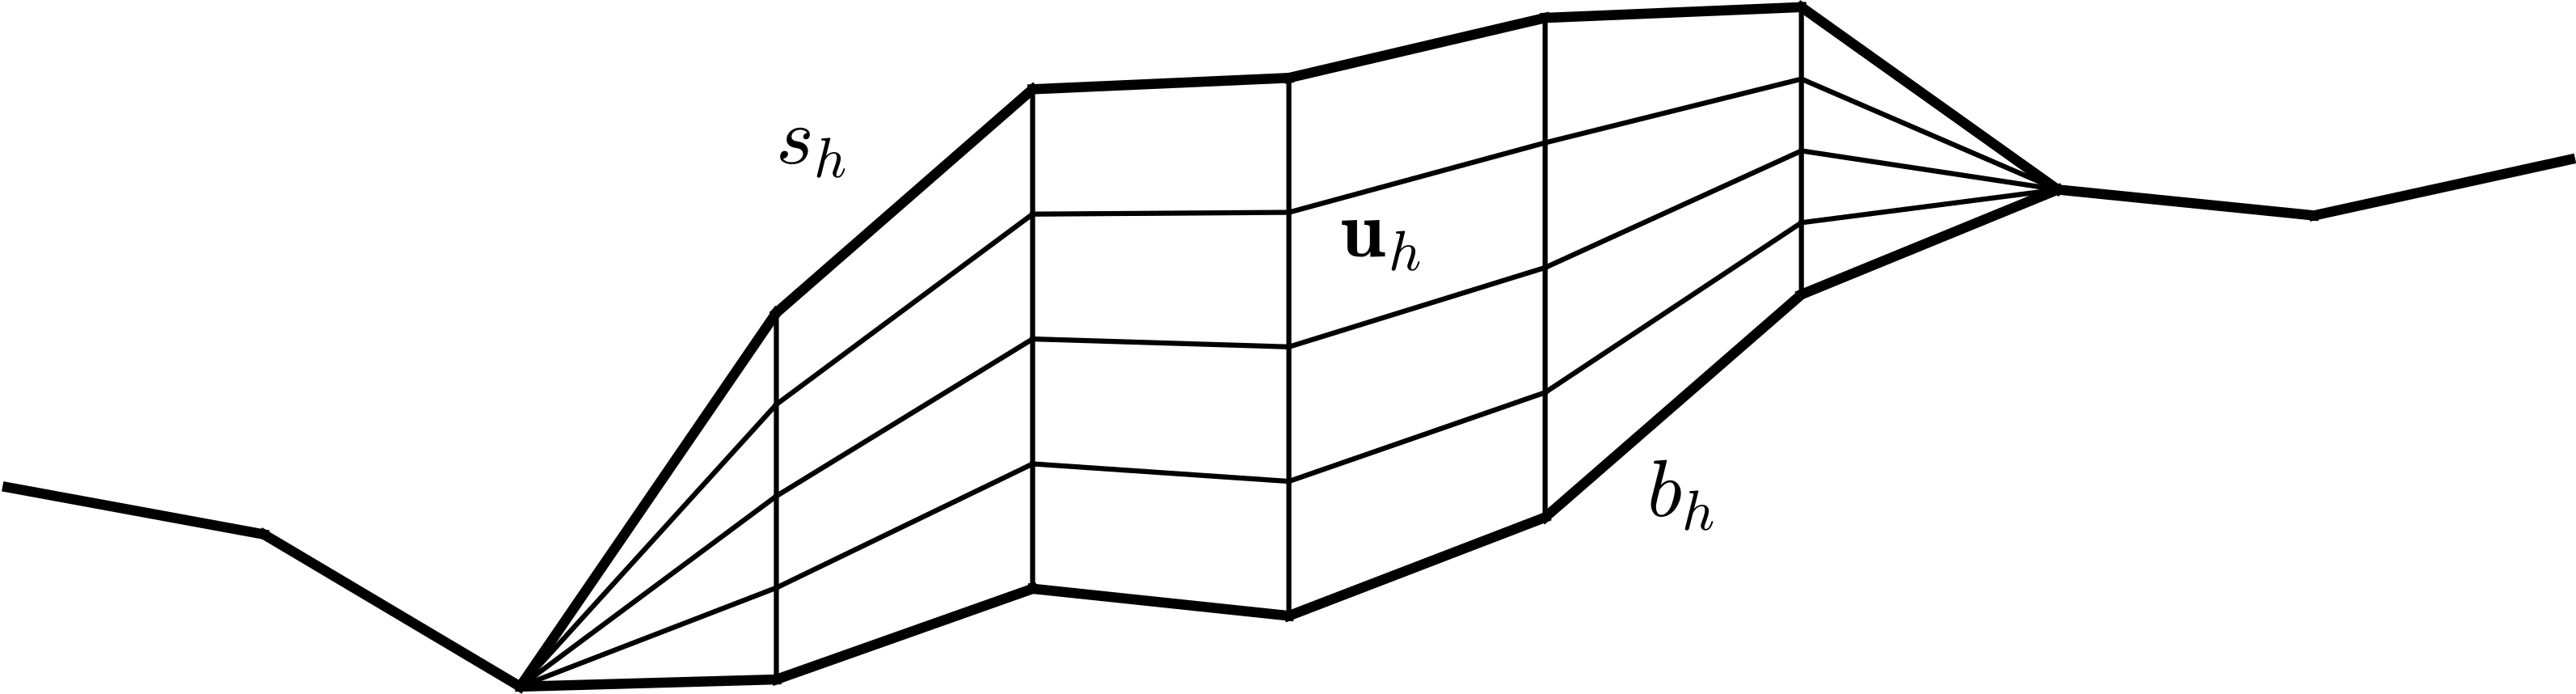
\includegraphics[width=0.7\textwidth]{genfigs/extruded.pdf}
\end{center}
\caption{Evaluating $F^h_{\Delta t}(s_h)$ in \eqref{eq:fe:be:vi} requires numerically (approximately) solving a Stokes problem on a mesh between $b_h$ and $s_h$, and then evaluating its upper surface trace: $\bu_h|_{s_h}$.}
\label{fig:fe:operatorvisualization}
\end{figure}

A key concern in applying abstract Theorem \ref{thm:abstractestimate}, or its Corollaries, in a glaciological context is the choice of the numerical bed elevation $b_h \approx b$, which defines the constraint set $\cK_h$.  First, we will assume that $b$ is continuous on the closed domain $\bar\Omega$, i.e.~$b\in C(\bar\Omega) \cap \cX$.  In practice $b$ is provided via a high resolution map derived from ice-penetrating radar \cite{Morlighemetal2017}, and it may already be in a continuous FE space, but often it is on a finer mesh than $\cT_h$.

We now assert that it is better to choose $b_h \in \cX_h$ to satisfy $b_h\ge b$ because the ``$\inf_{v\in\cK}$'' term in Section \ref{sec:abstractestimate} disappears; see Corollary \ref{cor:abstractestimate:nohull}.  A monotone nodal operator \eqref{eq:monotoneop}, or similar, can be applied to achieve this, $b_h = R^\oplus b$.  As one does in conforming FE methods for PDE problems \cite{Elmanetal2014}, we will also assume $b_h=b$ along the fixed boundary $\partial\Omega$.

Define an interpolation and truncation operation $\Pi_h : \cX \to \cK_h$ as follows.  For $r\in\cX$ this gives the unique FE function $\Pi_h(r) \in \cX_h$ so that
\begin{equation}
\Pi_h(r)(x_j) = \max \,\{b_h(x_j), r(x_j)\} \label{eq:definePi}
\end{equation}
for every interior node $x_j \in \cT_h$, with $\Pi_h(r)(x_j)=b(x_j)$ if $x_j\in\partial\Omega$.  Observe that definition \eqref{eq:definePi} only yields nodal admissibility.  The FE space must be such that this implies admissibility \emph{per se}, namely that $\Pi_h(r)(x) \ge b_h(x)$ for all $x \in \Omega$, so that $\Pi_h(r) \in \cK_h$.  This condition is satisfied by the continuous and piecewise-linear FE space $P_1$, but not, for example, by $P_2$ \cite{BuelerFarrell2024}, but compare the higher-order approach to FE solutions of VIs in \cite{KeithSurowiec2023}.

Collecting the above assumptions and context, from now on we make the following standard assumptions for solving VI problem \eqref{eq:be:vi} using numerical scheme \eqref{eq:fe:be:vi}.

\smallskip
\begin{stdass}
The following data are given:
\renewcommand{\labelenumi}{\arabic{enumi}.}
\begin{enumerate}
\item A bounded, convex polygon $\Omega\subset\RR^2$.
\item An exponent $\rr > 2$, with conjugate exponent $\rr' = \rr/(\rr-1)$. \label{item:rr}
\item A time-dependent SMB function $a\in C([0,T]; L^{\rr'}(\Omega))$.
\item A bed topography function $b \in C(\bar\Omega) \cap W^{1,\rr}(\Omega)$, with piecewise-linear boundary values $b|_{\partial\Omega}$.
\end{enumerate}
We make these definitions:
\begin{enumerate}
\setcounter{enumi}{4}
\item $\cX = W^{1,\rr}(\Omega)$, with the norm as defined in \eqref{eq:norm:Omega}.
\item $\cK = \{r\in\cX\,:\,r|_{\partial \Omega} = b|_{\partial \Omega} \text{ and } r \ge b\}$.
\item $\cX_h \subset \cX$ denotes a finite-dimensional and conforming FE space, from a mesh $\cT_h$ which exactly tiles $\bar\Omega$.
\end{enumerate}
The following are assumed to hold:
\begin{enumerate}
\setcounter{enumi}{7}
\item Conjecture \ref{conj:a}, with Lipschitz constant $\CA > 0$. \label{item:conj:a}
\item Conjecture \ref{conj:b}, with exponent $\qq>1$ and coercivity constant $\alpha > 0$.\label{item:conj:b}
\end{enumerate}
We also assume and define:
\begin{enumerate}
\setcounter{enumi}{9}
\item $b_h\in\cX_h$ is given, with $b_h\ge b$ on $\bar\Omega$ and $b_h=b$ along $\partial \Omega$. \label{item:goodbh}
\item $\cK_h = \{r_h\in\cX_h\,:\,r_h|_{\partial \Omega} = b_h|_{\partial \Omega} \text{ and } r_h \ge b_h\}$. \label{item:defineKh}
\item An interpolation/truncation operator $\Pi_h$ yielding admissible elements in $\cK_h$.  \label{item:Pi}
\end{enumerate}
\end{stdass}

\medskip
The conforming condition $\cK_h\subset \cK$ follows from assumptions \ref{item:goodbh} and \ref{item:defineKh}, with advantages to follow.  Note that defining $b_h=R^{\oplus} b$ implies assumption \ref{item:goodbh}, but we do not specifically assume this construction.  As seen in the proof of Theorem \ref{thm:stepwellposed}, assumptions \ref{item:conj:a} and \ref{item:conj:b} show that $F_{\Delta t}$ is $\qq$-coercive and Lipschitz on bounded subsets of $\cK$.  By Theorem \ref{thm:stepwellposed} and case \emph{i)} of Corollary \ref{cor:abstractestimate:nohull} we have the following Lemma.

\begin{lemma} \label{lem:preglacierapp}  Make the Standard Assumptions.  Suppose that $s^{n-1}\in\cK$ and define $\ell^n \in \cX'$ by \eqref{eq:be:source}.  Let $s\in\cK$ be the unique surface elevation satisfying the implicit time-step VI problem \eqref{eq:be:vi}, from Theorem \ref{thm:stepwellposed}.  Assume that $s_h\in\cK_h$ solves problem \eqref{eq:fe:be:vi}.  Let $R_h=\max\{\|s\|_\cX,\|s_h\|_\cX\}$.  Then there is a constant $c_0>0$, depending on $R_h$ and $\Delta t$, but not otherwise on $s$ or $s_h$, so that
\begin{align}
\|s-s_h\|_\cX^\rr &\le \quad \frac{2}{\alpha \Delta t} \inf_{r_h\in\cK_h} \left(F_{\Delta t}(s)-\ell^n\right)[r_h-s] \label{eq:preglacierestimate} \\
   &\quad\, + \frac{2}{\alpha \Delta t} \left(F_{\Delta t}(s_h)-F^h_{\Delta t}(s_h)\right)[s_h] \notag \\
   &\quad\, + c_0 \inf_{r_h\in\cK_h} \|r_h - s\|_{\cX}^\qq. \notag
\end{align}
\end{lemma}

Each term in estimate \eqref{eq:preglacierestimate} turns out to have a clear glaciological meaning, which we expose next.  Recall that $\cV=W_b^{1,\pp}(\Lambda(s_h); \RR^3)$ is the velocity space for the Stokes problem \eqref{eq:glenstokes:weak}, $h$ denotes the maximum diameter of cells in $\cT_h$, $\Lambda(s_h)$ denotes the 3D domain defined by $s_h$ using \eqref{eq:icydomain}, and $\tau_\pp(\Lambda(s_h))$ denotes the trace constant of that domain (Lemma \ref{lem:trace}).

\begin{theorem} \label{thm:glacierapp}  Make the Standard Assumptions.  Suppose that $s^{n-1}\in\cK$ and define $\ell^n \in \cX'$ by \eqref{eq:be:source}.  Let $s\in\cK$ be the unique solution of \eqref{eq:be:vi}, and $s_h\in\cK_h$ a solution of \eqref{eq:fe:be:vi}.  Define
\begin{equation}
\Omega_A(s) = \left\{x\in\Omega\,:\,s(x)=b(x)\right\},
\end{equation}
the active set for $s$, i.e.~the ice-free region for the exact solution.  Then
\begin{align}
\phantom{dfkljsd} \|s_h-s\|_\cX^\rr &\le \quad \frac{2}{\alpha \Delta t} \int_{\Omega_A(s)} (b - \ell^n) (b_h - b) &&\text{\textnormal{[term 1]}} \label{eq:glacierestimate} \\
   &\quad\, + \Gamma_{s_h} \big\|\bu_h - \bu\big\|_{\cV} &&\text{\textnormal{[term 2]}} \notag \\
   &\quad\, + c_0 \|\Pi_h(s) - s\|_\cX^\qq. &&\text{\textnormal{[term 3]}} \notag
\end{align}
The constant $c_0>0$ is from Lemma \ref{lem:preglacierapp}.  The coefficient in term 2, namely
\begin{equation}
\Gamma_{s_h} = \frac{c_1}{\alpha} \left(\frac{\tau_\pp(\Lambda(s_h))}{[H]}\right)^{1/\pp} \left(|\Omega| + [L]^{-\rr}\|s_h\|_{\cX}^\rr\right)^{1/(\pp'\rr)} \|s_h\|_{L^{\pp'\rr'}},
\end{equation}
depends nontrivially on $s_h$, but $c_1>0$ depends only on the exponents $\rr$, $\pp$.
\end{theorem}

Before proving the Theorem we sketch the meaning of each term, with further discussion after the proof.

\medskip
\begin{itemize}
\item[term 1:]  This term comes from FE approximation of the bed in the ice-free area $\Omega_A(s)$.  If the bed is exactly represented ($b_h=b$) then it is zero.  Note that $s_h \ge b_h \ge b = s$ in the ice-free area $\Omega_A(s)$, so the factor $b_h-b$ in the integrand reflects the smallest possible difference $s_h - s$.  Because $b-\ell^n\ge 0$ (Section \ref{sec:model}), the integrand is nonnegative.

\item[term 2:]  This term quantifies how numerical errors in solving the Stokes problem \eqref{eq:glenstokes:weak}, over the domain $\Lambda(s_h)$, will affect the geometrical error in $s_h$.

\item[term 3:]  An interpolation error term like this arises in the classical Cea's lemma argument for quasi-optimality of FE methods for PDEs \cite{Ciarlet2002}.  However, here the interpolant of $s$ is also truncated into $\cK_h$ using \eqref{eq:definePi}.
\end{itemize}

\begin{proof}  Because $s$ solves \eqref{eq:be:vi}, the residual $\Psi = F_{\Delta t}(s)-\ell^n \in \cX'$, while generally nonzero, is non-negative.  In fact, if $\phi\in C_c^\infty(\Omega)$ is nonnegative then $r=s+\phi \in \cK$ and $\Psi[r-s] = \Psi[\phi] \ge 0$.  Thus $\Psi\in\cX'$ is a non-negative distribution, and so it is represented by a positive Borel measure $\mu$ \cite[Theorem 6.22]{LiebLoss1997}, that is, $\Psi[\phi] = \int_\Omega \phi\,d\mu$.  However, by the proof of Theorem II.6.9 in \cite{KinderlehrerStampacchia1980} this measure is supported in $\Omega_A(s)$ and has density $b-\ell^n$ (Section \ref{sec:model}).

Now apply Lemma \ref{lem:preglacierapp}.  Note that $\bu|_{s}=\bzero$ and $s=b$ on $\Omega_A(s)$.  From the first term in \eqref{eq:preglacierestimate}, set $r_h = b_h \in \cK_h$ to give term 1:
\begin{equation}
\left(F_{\Delta t}(s)-\ell^n\right)[r_h-s] = \int_\Omega (b_h - s) \,d\mu = \int_{\Omega_A(s)} \left(b - \ell^n\right) (b_h - b).
\end{equation}

Consider the second term in \eqref{eq:preglacierestimate}.  Recall that $dS = |\bn_{s_h}|\,dx$ is the surface area element for the surface $\Gamma_{s_h} \subset \partial \Lambda(s_h)$.  After definitions \eqref{eq:be:Fdefine} and \eqref{eq:fe:be:Fdefine}, apply the triangle and H\"older inequalities:
\begin{align}
\left(F_{\Delta t}(s_h)-F^h_{\Delta t}(s_h)\right)&[s_h] = - \Delta t \int_\Omega \left(\bu|_{s_h} - \bu_h|_{s_h}\right)\cdot \bn_{s_h} s_h  \\
  &\le \Delta t \int_\Omega \Big|\bu|_{s_h} - \bu_h|_{s_h}\Big| |\bn_{s_h}|^{1/\pp} |\bn_{s_h}|^{1/\pp'} |s_h| \notag \\
  &\le \Delta t \left(\int_\Omega \Big|\bu|_{s_h} - \bu_h|_{s_h}\Big|^\pp |\bn_{s_h}|\right)^{1/\pp} \left(\int_\Omega |\bn_{s_h}| |s_h|^{\pp'}\right)^{1/\pp'} \notag \\
  &\le \Delta t \left(\int_{\Gamma_{s_h}} \big|\bu - \bu_h\big|^\pp dS\right)^{1/\pp} \left(\int_\Omega |\bn_{s_h}|^\rr\right)^{1/(\pp'\rr)} \|s_h\|_{L^{\pp'\rr'}} \notag
\end{align}
Now apply the trace inequality (Lemma \ref{lem:trace}) and use the facts that $\rr>2$ and $(1+\alpha)^{\rr/2} \le 2^{(\rr-2)/2} (1+\alpha^{\rr/2})$ if $\alpha\ge 0$:
\begin{align}
\left(F_{\Delta t}(s_h)-F^h_{\Delta t}(s_h)\right)[s_h] &\le \Delta t \left(\frac{\tau_\pp(\Lambda(s_h))}{[H]}\right)^{1/\pp} \|\bu - \bu_h\|_{\cV} \\
  &\qquad \cdot \left(2^{(\rr-2)/2} \int_\Omega 1 + |\grad s_h|^\rr\right)^{1/(\pp'\rr)} \|s_h\|_{L^{\pp'\rr'}}.  \notag
\end{align}
Recalling norm definition \eqref{eq:norm:Omega}, we have term 2.

Term 3 follows by substituting $r_h=\Pi_h(s)$ into the third term in \eqref{eq:preglacierestimate}.
\end{proof}

Regarding term 1, consider those portions of $\Omega_A(s)$ which are also ice-free according to the FE solution, namely points $x \in \Omega_A(s) \cap \Omega_A^h(s_h)$ where $\Omega_A^h(s_h) = \{x\in\Omega\,:\,s_h(x)=b_h(x)\}$.  In such areas generally $b_h > b$, for example because of the monotone restriction used for assumption \ref{item:goodbh}.  This implies that there is a positive ``fake ice thickness'' error for the FE solution, namely $s_h - b=b_h-b>0$.  However, the numerical model reports zero thickness ($s_h-b_h=0$).  In areas of strong ablation, and far from the nearest flowing glacier, one might simply declare that such ``fake ice'' does not represent an FE-generated error.  Then the magnitude of term 1 can be reduced accordingly, by excluding obviously ice-free areas from the integral.  However, generally $s$ is unknown.  In fact, such exclusion is apparently not implementable near the unknown free boundary $\Omega \cap \partial \Omega_A(s)$.

Note that a time-stepping FE solution of any fluid-layer VI problem like \eqref{eq:be:vi} commits a mass conservation error near the (unknown) exact free boundary even when there is no difference between the exact and FE obstacles.  The mass conservation barrier theory in \cite{Bueler2021conservation} addresses this concern, in terms of the fluid layer thickness, thus in in a case where the obstacle is the zero function, which has an exact FE representation.  While the theory in \cite{Bueler2021conservation} applies here as well, term 1 in bound \eqref{eq:glacierestimate} is new relative to the various mass-conservation errors identified in \cite{Bueler2021conservation}.

The Stokes velocity error norm $\|\bu_h - \bu\|_{\cV}$ in term 2 of \eqref{eq:glacierestimate} describes the error in solving problem \eqref{eq:glenstokes:weak} on a particular 3D domain $\Lambda(s_h)$.  If one supposes counter-factually that $\Lambda(s_h)$ does not change under mesh refinement, then one may use reasonable assumptions and existing techniques to derive a convergence rate for this term.  The following sketch from \cite[Theorem 4.9]{JouvetRappaz2011} does this; see also the FE theory for linear Stokes in \cite{Elmanetal2014}.  One assumes solution regularity for the Stokes problem \eqref{eq:glenstokes:weak}, specifically that $\bu\in W^{2,\kappa}(\Lambda(s_h);\RR^3)$ and $p \in W^{1,\kappa'}(\Lambda(s_h))$ for some $\kappa \in [\pp,2]$.  The mixed FE method for \eqref{eq:glenstokes:weak} is assumed to satisfy Bramble-Hilbert interpolation bounds in $W^{1,\kappa}(\Lambda(s_h))$ and $L^{\kappa'}(\Lambda(s_h))$ for the discrete velocity and pressure spaces, respectively; see \cite[inequalities (4.26), (4.27)]{JouvetRappaz2011}.  Finally one assumes that the mixed FE method satisfies a discrete inf-sup condition \cite[equation (4.1)]{JouvetRappaz2011}.  One then concludes with a convergence rate, $\|\bu_h - \bu\|_{\cV} \le C h^{\kappa/2}$, for a constant $C>0$ which depends on the regularity norms of $\bu,p$, the discrete inf-sup constant, and the domain $\Lambda(s_h)$.

To apply such a technique to bounding term 2 of \eqref{eq:glacierestimate} in Theorem \ref{thm:glacierapp}, in the realistic context of VI problem \eqref{eq:be:vi}, one would at least need to prove two new bounds.  First, one would need a bound showing the regularity of the solution $\bu,p$ of \eqref{eq:glenstokes:weak}, over the domain $\Lambda(s_h)$, when $s_h \in \cX_h \subset W^{1,\rr}(\Omega)$; this extends Conjecture \ref{conj:a}.  Second, seemingly much more difficult, one would need to bound how the constant in the convergence rate ``$C h^{\kappa/2}$'' (previous paragraph) depends on the properties of $\Lambda(s_h)$.

One might also try to bound term 3 in \eqref{eq:glacierestimate} via estimates for FE interpolation.  From \cite[Theorem 3.1.6]{Ciarlet2002}, for example, if $\mu \in [\rr,+\infty]$ then there is $C>0$, depending only on the finite element family for $\cX_h$, such that for all $r \in W^{2,\mu}(\Omega)$,
\begin{equation}
\|\pi_h(r) - r\|_{\cX} \le C h |\Omega|^{(1/\rr)-(1/\mu)} \|r\|_{W^{2,\mu}}. \label{eq:ciarletregularity}
\end{equation}
Here $\pi_h$ is the ordinary interpolation into $\cX_h$, not including truncation into $\cK_h$ as in operation \eqref{eq:definePi}.

Now suppose we somehow arrange that $\cK_h=\cK$, thus that $\Pi_h=\pi_h$, and suppose also that the exact solution $s\in\cK$ of VI problem \eqref{eq:be:vi} satisfies $s\in W^{2,\mu}(\Omega)$ for some $\mu \in [\rr,+\infty]$.  Then it follows that term 3 in \eqref{eq:glacierestimate} is $O(h)$ with a coefficient that depends on the $W^{2,\mu}$ norm of $s$.  The argument for \cite[Theorem 4.3]{JouvetBueler2012} makes a comparably-strong regularity assumption for a power of the thickness function in an SIA problem.

However, the sketch in the previous paragraph is largely a fantasy.  The hypothesis that $s\in W^{2,\mu}(\Omega)$ is too strong even if the data $a,b$ entering into VI problem \eqref{eq:be:vi} are arbitrarily smooth.  While it is true that in classical obstacle problems the solution is generically tangential along the free boundary, which permits such regularity \cite[Chapter IV]{KinderlehrerStampacchia1980}, here a glacier's surface gradient need not approach the bed gradient at points along the ice margin (Subsection \ref{subsec:margin}).  Thus, while $s \in \cX = W^{1,\rr}(\Omega)$ is credible, $s\in W^{2,\mu}(\Omega)$ is probably not.  Direct use of standard FE interpolation theory to prove convergence from a result like Theorem \ref{thm:glacierapp} would seem to be difficult.


\section{Discussion and conclusion} \label{sec:conclusion}

The major result of this paper is Theorem \ref{thm:glacierapp}, which bounds the numerical surface elevation error when a glacier is modeled using non-shallow Stokes dynamics.  The bound, inequality \eqref{eq:glacierestimate}, only estimates the FE error made in a single implicit time step, namely VI problem \eqref{eq:be:vi}.  The first two terms in the bound can be reduced by improving bed elevation interpolation, and by solving the Stokes problem more accurately, respectively.

All terms in bound \eqref{eq:glacierestimate} would be reduced by increased mesh resolution.  However, the surface elevation solution to \eqref{eq:be:vi} must be expected to have low regularity, especially across the ice margin (free boundary); see Subsection \ref{subsec:margin}.  Near-margin mesh refinement may be the only technique which reduces the interpolation/truncation error in the surface elevation, i.e.~term 3 in \eqref{eq:glacierestimate}.

Thus the results here leave us far from an FE convergence proof for the main time-evolution problem of glaciology, which is written the Introduction.  This problem couples NCP \eqref{eq:ncp} to the Stokes problem \eqref{eq:glen}--\eqref{eq:stokes}.  It is a (roughly) parabolic VI \cite{Glowinski1984}, on which analysis is generally more difficult than for the (roughly) elliptic single-step VI problem \eqref{eq:be:vi}.  Converting Theorem \ref{thm:glacierapp} to a convergence proof for the time-dependent theory would require significant extensions.

Neither do we have a proof of the well-posedness of the continuous-space, implicit-step problem \eqref{eq:be:vi} itself.  Much of the current paper is devoted to conjecturing such well-posedness (Sections \ref{sec:model}--\ref{sec:numerical}).  The abstract FE bound in Theorem \ref{thm:abstractestimate} applies to problem \eqref{eq:be:vi} because of Theorem \ref{thm:stepwellposed}, an immediate consequence of Conjectures \ref{conj:a} and \ref{conj:b}.  On the other hand, our attempt here at least clarifies which properties of the surface motion, i.e.~as part of the surface kinematical equation free-boundary problem, need to hold to conclude well-posedness of the time step problems in a non-shallow glacier model.

The heart of the matter is coercivity of the surface motion, namely Conjecture \ref{conj:b}.  A strategy for proving this Conjecture is not clear to this author.  A weaker version comes from setting $r=s + \eps\phi$ for $\phi$ supported where $s>b$.  That is, one could consider admissible perturbations of the glacier surface which do not move the glacier margin.  This may be easier to prove, but it is not sufficient for Theorem \ref{thm:stepwellposed}, and it does not address the marginal shape and overhang concerns in Subsection \ref{subsec:margin}.  On the other hand, one might modify or regularize the operator definition \eqref{eq:be:Fdefine} in some manner, e.g.~by adding an elliptic regularization term.  Our numerical evidence for coercivity of the existing operator, from a very basic numerical approach, is weak (Section \ref{sec:numerical}), but in a regularized model the near-margin numerical approximation might be easier and the coercivity more evident.

%\clearpage\newpage
\bibliographystyle{siamplain}
\bibliography{estimate}

\appendix
\section{Proof of Lemma \ref{lem:stokesapriori}} \label{app:provestokesapriori}

The proof of Lemma \ref{lem:stokesapriori} is hinted in \cite{JouvetRappaz2011}, and is standard.  It requires Poincar\'e's inequality, below as \eqref{eq:poincare}, which is (7.44) in \cite{GilbargTrudinger2001}, and Korn's inequality \eqref{eq:korns}, which can by proven by setting $F(x)$ to the identity in Corollary 4.1 of \cite{Pompe2003}.

\begin{lemma} \label{lem:poincarekorns}
Under the assumptions of Theorem \ref{thm:stokeswellposed}, there exist dimensionless constants $C$, depending on the geometry of $\Lambda$, so that for all $\bv \in \cV$,
\begin{equation}
\int_\Lambda |\bv|^\pp \le C [H]^\pp \int_\Lambda |\grad\bv|^\pp, \label{eq:poincare}
\end{equation}
thus $\|\bv\|_{\cV}^\pp \le (C + 1) [H]^\pp \int_\Lambda |\grad\bv|^\pp$, and
\begin{equation}
\int_\Lambda |\grad\bv|^\pp \le C \int_\Lambda |D\bv|^\pp. \label{eq:korns}
\end{equation}
\end{lemma}

\begin{proof}[Proof of Lemma \ref{lem:stokesapriori}]
From \eqref{eq:glenstokes:weak} and $\bu \in\Vdiv$ it follows that
\begin{equation}
0= F_\Lambda(\bu,p)[\bu,p] = \int_\Lambda 2 \nu(D\bu) D\bu : D\bu - \rhoi \bg \cdot \bu.  \label{eq:stokes:substituteu}
\end{equation}
Apply \eqref{eq:korns}, the facts that $\pp>0$ and $(\pp-2)/2 \le 0$, and equation \eqref{eq:glen}:
\begin{align}
\int_\Lambda |\grad\bu|^\pp &\le C \int_\Lambda |D\bu|^\pp \le C \int_\Lambda \left(|D\bu|^2 + \eps\right)^{(\pp-2)/2} \left(D\bu:D\bu + \eps\right) \label{eq:stokes:startapriori} \\
	&= C \left[\eps^{\pp/2} |\Lambda| + (2 \nu_\pp)^{-1} \int_\Lambda 2\nu(D\bu) D\bu:D\bu\right]. \notag
\end{align}
By equation \eqref{eq:stokes:substituteu}, Cauchy-Schwarz, and H\"older's inequality we thus have
\begin{align}
\int_\Lambda |\grad\bu|^\pp &\le C \left[\eps^{\pp/2} |\Lambda| + (2 \nu_\pp)^{-1} \int_\Lambda \rhoi \bg \cdot \bu\right] \label{eq:stokes:workapriori} \\
	&\le C \left[\eps^{\pp/2} |\Lambda| + (2 \nu_\pp)^{-1} \rhoi |\bg| |\Lambda|^{1/\pp'} \|\bu\|_\cV\right]. \notag
\end{align}
From \eqref{eq:poincare},
\begin{equation}
\|\bu\|_{\cV}^\pp \le C [H]^\pp \left[\eps^{\pp/2} |\Lambda| + (2 \nu_\pp)^{-1} \rhoi |\bg| |\Lambda|^{1/\pp'} \|\bu\|_\cV\right].
\end{equation}
Now let $z=\|\bu\|_\cV$.  We have proved that $z^\pp \le c_0 + c_1 z$ for $\pp>1$ and constants $c_i>0$.  Furthermore $g(y) = y^\pp - c_1 y - c_0$ is smooth with $g(0)=-c_0<0$, and $g(y) \to +\infty$ as $y \to +\infty$ since $\pp>1$.  Thus there exists a right-most root $\tilde y>0$ with $\tilde y = f(\pp,c_0,c_1)$.  Since $g(z)\le 0$ we have $z \le \tilde y$.  This proves \eqref{eq:stokesapriori} with $C=\tilde y$.
\end{proof}
\end{document}
